\documentclass[12pt,a4paper]{report}

\usepackage{iftex}
\ifPDFTeX
\usepackage[T1]{fontenc}
\usepackage[utf8]{inputenc}
\usepackage{lmodern}
\fi
\usepackage[english]{babel}
\usepackage{geometry}
\usepackage{setspace}
\usepackage{microtype}
\usepackage{graphicx}
\usepackage{booktabs}
\usepackage{rotating}
\usepackage{pdflscape}
\usepackage{tabularx}
\usepackage{amsmath}
\usepackage{amssymb}
\usepackage{siunitx}
\usepackage{csquotes}
\usepackage[numbers,sort&compress]{natbib}
\usepackage{hyperref}

% NCAL LaTeX theme colors and cover-page helpers.
% The alpha channel from the provided hex codes is omitted because the values are fully opaque.

\usepackage{xcolor}
\usepackage{tikz}
\usepackage{titlesec}
\usetikzlibrary{calc,fadings}

\ifPDFTeX\else
\usepackage{fontspec}
\defaultfontfeatures{Ligatures=TeX,Scale=MatchLowercase}

\setmainfont{Urbanist}[
  Path=fonts/Urbanist/,
  UprightFont=Urbanist[wght].ttf,
  ItalicFont=Urbanist-Italic[wght].ttf,
  BoldFont=Urbanist[wght].ttf,
  BoldItalicFont=Urbanist-Italic[wght].ttf,
  UprightFeatures={RawFeature={axis={wght=400}}},
  ItalicFeatures={RawFeature={axis={wght=400}}},
  BoldFeatures={RawFeature={axis={wght=700}}},
  BoldItalicFeatures={RawFeature={axis={wght=700}}}
]

\setsansfont{Urbanist}[
  Path=fonts/Urbanist/,
  UprightFont=Urbanist[wght].ttf,
  ItalicFont=Urbanist-Italic[wght].ttf,
  BoldFont=Urbanist[wght].ttf,
  BoldItalicFont=Urbanist-Italic[wght].ttf,
  UprightFeatures={RawFeature={axis={wght=400}}},
  ItalicFeatures={RawFeature={axis={wght=400}}},
  BoldFeatures={RawFeature={axis={wght=700}}},
  BoldItalicFeatures={RawFeature={axis={wght=700}}}
]

\setmonofont{Latin Modern Mono}[Scale=MatchLowercase]
\fi

\definecolor{NCALPrimary}{HTML}{071C33}
\definecolor{NCALSecondary}{HTML}{E78861}
\definecolor{NCALWhite}{HTML}{FFFFFF}
\definecolor{NCALBlack}{HTML}{000000}

\hypersetup{
  colorlinks=true,
  linkcolor=NCALPrimary,
  citecolor=NCALSecondary,
  urlcolor=NCALPrimary
}

\titleformat{\chapter}[display]
  {\normalfont\bfseries\color{NCALPrimary}}
  {\filleft\Large\color{NCALSecondary}\chaptername\ \thechapter}
  {0.8ex}
  {\filright\Huge}
  [\vspace{0.8ex}\titlerule]

\titlespacing*{\chapter}{0pt}{0pt}{24pt}

\titleformat{\section}
  {\normalfont\Large\bfseries\color{NCALPrimary}}
  {\thesection}{0.8em}{}

\titleformat{\subsection}
  {\normalfont\large\bfseries\color{NCALPrimary}}
  {\thesubsection}{0.8em}{}

\newcommand{\NCALInstitute}{NPI, \'UJV \v{R}e\v{z}}

\makeatletter
\newcommand{\NCALCoverPage}{%
  \begin{titlepage}
    \newgeometry{margin=0pt}
    \pagecolor{NCALPrimary}
    \thispagestyle{empty}
    \begin{tikzpicture}[remember picture,overlay]
      % Solid background
      \fill[NCALPrimary] (current page.south west) rectangle (current page.north east);

      % Hero aerial photo – cropped to the frame without distorting the panorama.
      \begin{scope}
        \clip (current page.north west) rectangle ($(current page.north east)+(0,-0.38\paperheight)$);
        \node[anchor=north,inner sep=0pt] at (current page.north) {%
          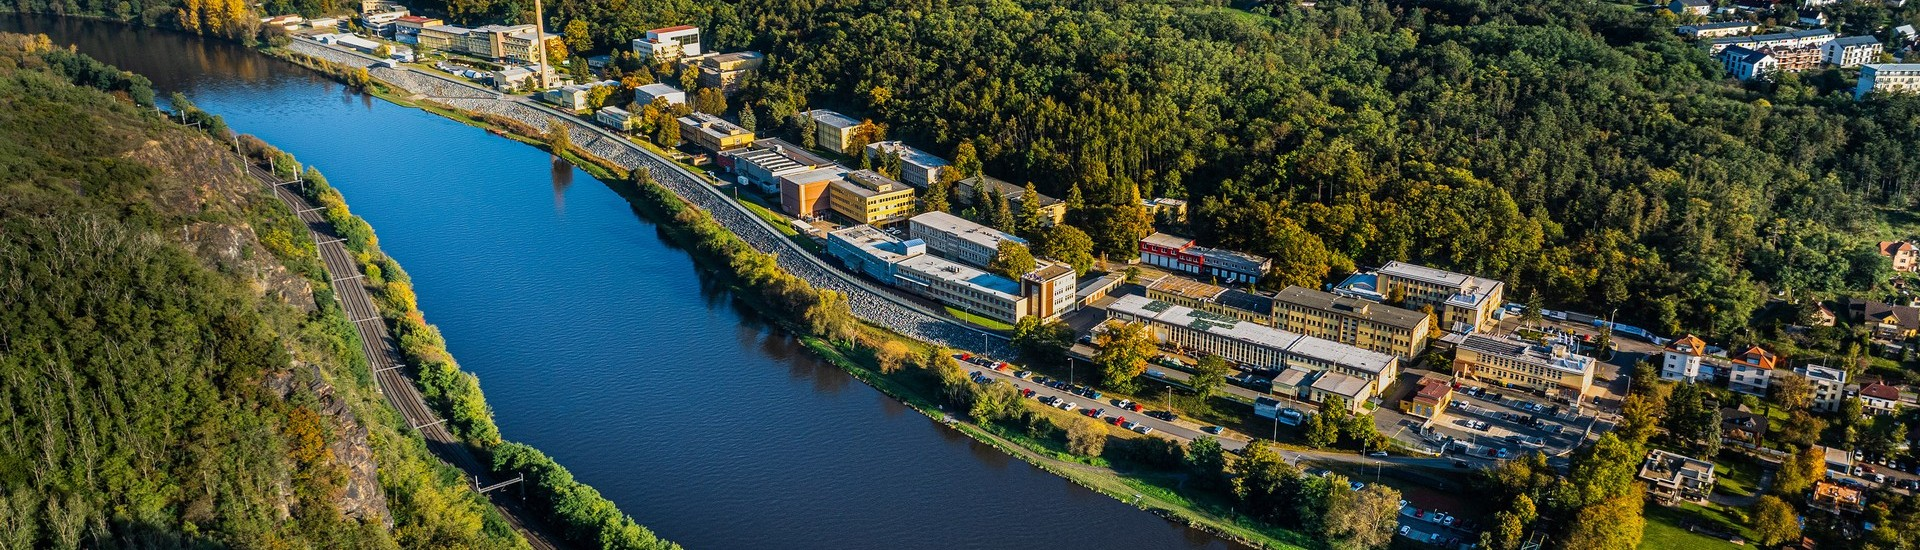
\includegraphics[height=0.38\paperheight]{figures/ujv_jaderne-udoli_dron_2024_3_4k.jpg}%
        };
      \end{scope}

      % Gradient fade from photo into NCALPrimary
      \fill[NCALPrimary, path fading=north]
        ($(current page.north west)+(0,-0.22\paperheight)$)
        rectangle
        ($(current page.north east)+(0,-0.40\paperheight)$);

      % Long NCALSecondary divider with equal page margins.
      \fill[NCALSecondary]
        ($(current page.north west)+(0.085\paperwidth,-0.555\paperheight)$)
        rectangle ++(0.83\paperwidth,0.0028\paperheight);

      % ---- Title block ----
      \node[
        anchor=north west,
        text width=0.62\paperwidth,
        align=left,
        text=NCALWhite
      ] at ($(current page.north west)+(0.085\paperwidth,-0.58\paperheight)$) {%
        {\fontsize{28}{34}\selectfont\bfseries
          NCAL Characterization\par}
        \vspace{0.42em}
        {\fontsize{18.5}{23}\selectfont\bfseries
          at \NCALInstitute\par}
        \vspace{0.55em}
        {\fontsize{14}{18}\selectfont\color{NCALSecondary}\bfseries
          Working Document\par}
        \vspace{1.7em}
        {\fontsize{12}{16}\selectfont \@author\par}
        \vspace{0.3em}
        {\fontsize{10.5}{14}\selectfont\color{NCALWhite!65!NCALPrimary}
          \NCALInstitute\par}
        \vspace{0.3em}
        {\fontsize{10.5}{14}\selectfont\color{NCALWhite!65!NCALPrimary}
          \@date\par}
      };

      % ---- NCAL detector photo – larger, right-aligned, centered on the Rez image baseline ----
      \node[anchor=east, inner sep=2.5pt,
            fill=NCALWhite,
            draw=NCALSecondary, line width=1pt]
        at ($(current page.north east)+(-0.085\paperwidth,-0.38\paperheight)$) {%
          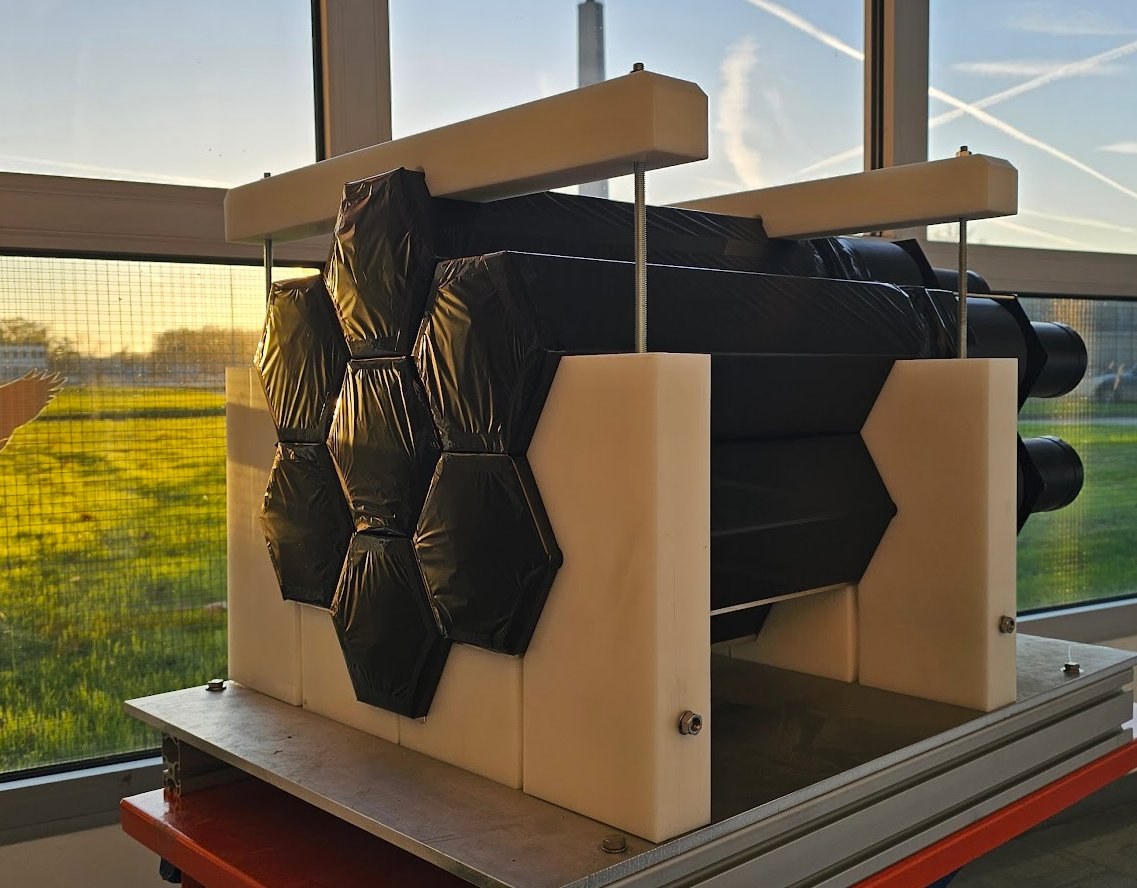
\includegraphics[width=0.24\paperwidth]{figures/NCAL.jpg}%
        };

      % ---- Bottom-right collaborator badge ----
      \fill[NCALSecondary]
        ($(current page.south east)+(-0.280\paperwidth,0.105\paperheight)$)
        rectangle ++(0.195\paperwidth,0.0015\paperheight);

      \node[anchor=south east,
            text=NCALWhite!50!NCALPrimary,
            font=\fontsize{6.8}{8}\selectfont]
        at ($(current page.south east)+(-0.085\paperwidth,0.109\paperheight)$) {%
          {\addfontfeatures{LetterSpace=4.0}COLLABORATING INSTITUTIONS}};

      \fill[NCALWhite, rounded corners=3pt]
        ($(current page.south east)+(-0.280\paperwidth,0.058\paperheight)$)
        rectangle ++(0.195\paperwidth,0.024\paperheight);

      \node[anchor=center]
        at ($(current page.south east)+(-0.1825\paperwidth,0.070\paperheight)$) {%
          
\includegraphics[width=0.182\paperwidth,trim=17 5 20 7,clip]{figures/collaborators.png}%
        };
    \end{tikzpicture}

    \null
  \end{titlepage}%
  \nopagecolor
  \restoregeometry
}
\makeatother

\newcolumntype{Y}{>{\raggedright\arraybackslash}X}

\geometry{margin=2.8cm}
\onehalfspacing

\title{NCAL Characterization at \NCALInstitute\\Working Document}
\author{Dachi Okropiridze}
\date{April 2026}

\begin{document}

\pagenumbering{gobble}
\NCALCoverPage
\clearpage
\pagenumbering{roman}
\tableofcontents
\clearpage
\pagenumbering{arabic}

\chapter{Introduction}

\section{Physics and detector context}

The Compressed Baryonic Matter (CBM) experiment at FAIR is designed to study strongly interacting matter at high net-baryon density under laboratory conditions \citep{Friman2011CBMPhysicsBook}. Within that program, reliable event characterization is essential: centrality determination, reaction-plane reconstruction, and the interpretation of event-by-event observables all depend on a robust measurement of forward-going spectator matter. The forward detector system therefore has a direct impact on the quality of the physics extracted from heavy-ion data, especially in the high-rate environment foreseen for CBM.

The Forward Spectator Detector (FSD) has been developed as the dedicated forward detector for spectator nucleons and nuclear fragments in CBM. Its role is to provide event-plane information and support centrality reconstruction at the interaction rates relevant for the experiment \citep{Dvorak2025FSD}. However, charged spectators alone do not provide the full picture of the forward final state. A measurement of neutral forward particles, especially neutrons, is required if the forward system is to deliver a more complete description of spectator emission and its correlation with the collision geometry.

The Neutron Calorimeter (NCAL) addresses this missing neutral component. According to the current NCAL addendum, the detector is intended to complement the FSD by measuring forward neutral spectators and thereby strengthening centrality and collective-flow related measurements in the CBM heavy-ion program \citep{Okropiridze2026NCALAddendum}. The same document also emphasizes a broader physics reach: forward neutron detection can support dedicated studies of elementary channels such as proton-proton and deuteron-proton reactions, and may provide a handle for initial-state neutron tagging in deuteron-induced interactions \citep{Okropiridze2026NCALAddendum}. In that sense, NCAL is not merely an auxiliary subsystem, but a detector with its own performance questions and physics potential.

The present NCAL prototype program is built around repurposed detector components originating from the COSY Time-of-Flight system, combined into dedicated test configurations for commissioning and performance studies \citep{Okropiridze2024SimulationNCAL,Okropiridze2026NCALAddendum}. Prototype setups have been used both in the mini-CBM environment at GSI and in external test campaigns, including measurements at \NCALInstitute \citep{Okropiridze2026NCALAddendum}. These campaigns are scientifically important because they provide controlled conditions under which detector response can be studied before the final integration of NCAL into the CBM forward system.

\section{Motivation for the present study}

The main objective of the present work is to characterize the NCAL prototype at a level that is useful for detector development, future integration, and later publication. In practical terms, this means quantifying how the detector responds in a neutron-beam environment, identifying which observables carry the strongest discriminating power, and determining which aspects of the readout chain are stable enough to support reproducible analysis.

One central question is the neutron detection efficiency of the detector under the beam conditions available during the test campaign. That quantity is directly relevant for evaluating whether the prototype geometry, active material, and readout concept are adequate for the role envisioned for NCAL in the CBM forward system. Efficiency, however, is not the only quantity of interest. A useful neutron detector must also be understood in terms of timing behavior, prompt backgrounds, and event-selection quality. For that reason, the present study also treats particle-identification methods as a core topic rather than a secondary analysis exercise.

The detector-development aspect of this work is equally important. The campaign is not only a neutron-response measurement; it is also a test bench for readout and data-acquisition concepts. In particular, the study is intended to improve the understanding of NCAL performance when operated with the newly developed DOGMA front-end electronics and with the older DiRICH-based chain used in earlier detector work. Even when the final CBM readout choice lies outside the scope of this document, comparative operation with these chains is highly informative because it exposes differences in timing reference quality, signal handling, data integrity, and downstream analysis requirements. A careful comparison is therefore part of understanding the detector itself. The second campaign at \NCALInstitute should therefore be understood primarily as a detector-characterization and readout-validation experiment rather than as a finalized production-data run.

\subsection{Motivation from the first campaign at \NCALInstitute}

The present campaign should be read explicitly as experiment~2. According to the current run history, the preceding campaign used a proton-on-lithium neutron-production target in a fixed-position configuration. In that first experiment, the gamma-induced population formed a broad structure directly beneath the neutron-candidate region in the time-of-flight versus pulse-height plane. Under those conditions, the overlap between the two populations made it very difficult to characterize the NCAL detector response cleanly.

Figure~\ref{fig:rez1-gamma-neutron-overlap} documents that limitation using the time-of-flight-overlay version of the first-campaign plot. The figure is included here because it captures the central practical reason for carrying out a second campaign under modified conditions: the dominant lower population and the neutron-candidate accumulation were not sufficiently separated in the observable space available in experiment~1. For comparison, the same figure also includes an analytical estimate of the prompt-gamma and \SI{30}{MeV} neutron time-of-flight dependence on detector distance, together with the corresponding time-of-flight difference.

\begin{figure}[tbp]
\centering
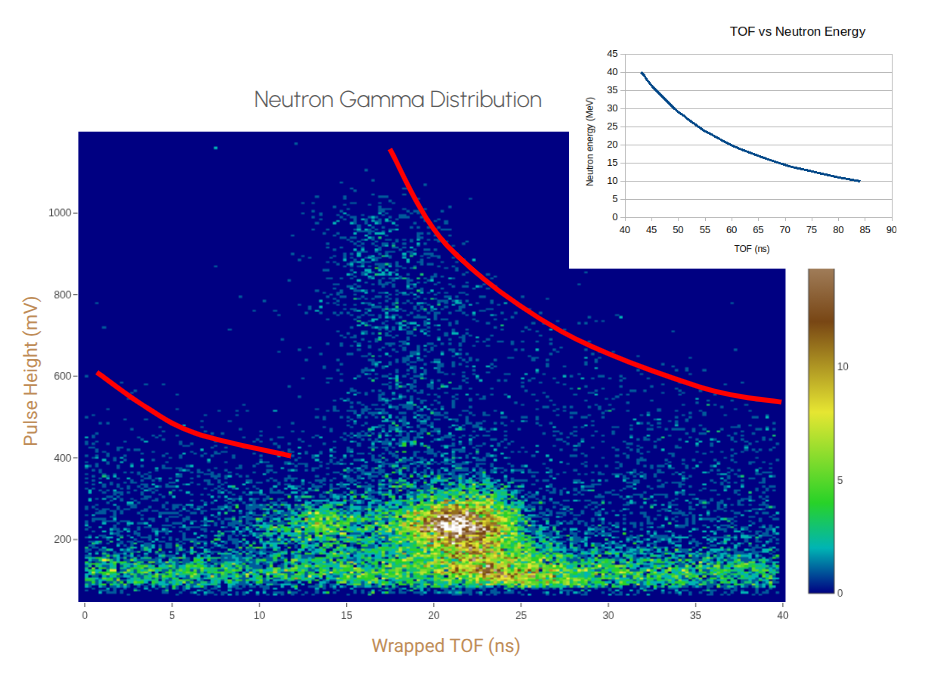
\includegraphics[width=0.88\textwidth,height=0.34\textheight,keepaspectratio]{figures/NCAL_Gamma_NEutron_hist_REZ1_TOFoverlay.png}

\vspace{0.8em}

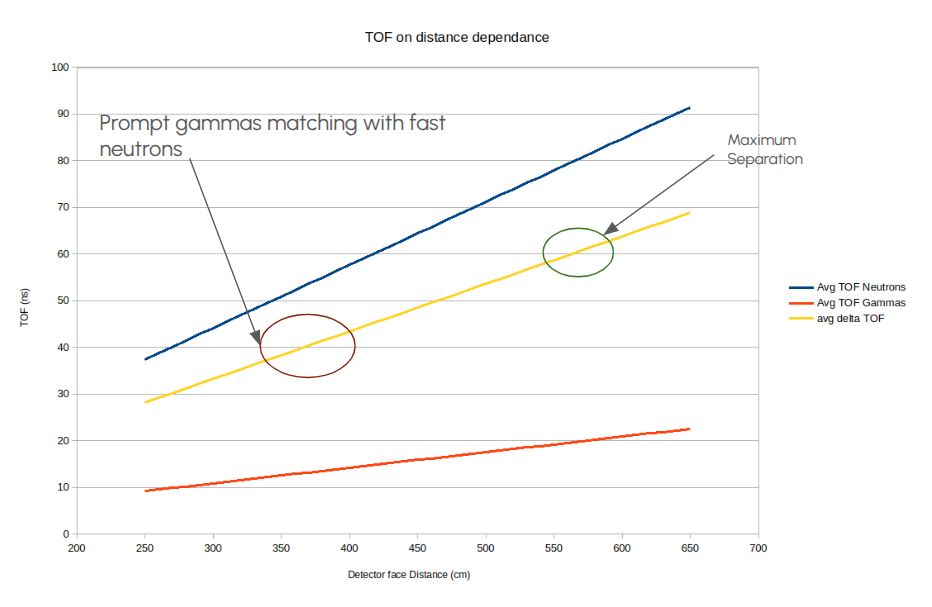
\includegraphics[width=0.88\textwidth,height=0.34\textheight,keepaspectratio]{figures/Gamma_Neutron_deltaTOF_30MeVneutrons.png}
\caption{Top: wrapped time-of-flight versus pulse-height distribution from the first campaign at \NCALInstitute, shown in the time-of-flight-overlay form used during later interpretation of the dataset. In the working interpretation of experiment~1, the broad lower population corresponds to gamma-induced events, while the higher-time-of-flight structure contains the neutron-candidate region. Bottom: analytical estimate of prompt-gamma time of flight, \SI{30}{MeV} neutron time of flight, and the corresponding time-of-flight difference as a function of detector-face distance. Together, the two panels illustrate why limited timing separation in the first campaign made a clean characterization of the NCAL response difficult.}
\label{fig:rez1-gamma-neutron-overlap}
\end{figure}

\section{Scope of this document}

This document is being developed as a broad scientific record of the second experimental campaign and is intended to mature into material suitable for a thesis chapter and, after further refinement, parts of one or more journal articles. Its purpose is therefore twofold. First, it should document the experiment rigorously enough that the measurement logic, detector configuration, and analysis choices remain transparent and reproducible. Second, it should separate verified results from working hypotheses, so that later interpretation can be strengthened without rewriting the experimental history.

The analysis workflow already points toward the structure needed for such a document. The existing event-digestion tools extract trigger-referenced observables such as leading and trailing edge times, time-over-threshold values, trigger-to-trigger spacing, and timing jitter from raw DOGMA-formatted data. These observables are natural building blocks for beam-structure studies, time-of-flight analysis, and future particle-identification strategies. Accordingly, the full document should evolve toward a coherent treatment of the experimental setup, beam conditions, detector geometry, veto configuration where applicable, DAQ architecture, calibration logic, event reconstruction, uncertainty sources, and performance observables.

At the present stage, the introduction is intentionally conservative. It establishes the detector and physics context from available project documents and defines the immediate scientific aims of this campaign: characterization of NCAL, evaluation of neutron-response observables, exploration of PID strategies, and assessment of detector operation together with DOGMA and DiRICH readout concepts. Subsequent chapters can build on this foundation by adding the finalized beamline description, analysis methodology, efficiency extraction strategy, uncertainty treatment, and validated experimental results.
\chapter{Experimental Setup}

The second NCAL campaign at \NCALInstitute was carried out in the proton-driven neutron environment of the U-120M cyclotron. This chapter summarizes the experimental arrangement relevant for interpreting detector response: the beamline geometry, detector placement, shielding layout, and the roles of the main supporting subsystems. Detailed source-reaction physics is treated in the next chapter, while detector construction and DAQ implementation are described later.

\section{Setup geometry and detector placement}

Figure~\ref{fig:rez2-working-setup} summarizes the layout adopted for experiment~2. The schematic records the current setup logic, detector ordering, and monitoring strategy along the beam axis, while also identifying those elements that remained under optimization during preparation of the campaign.

\begin{figure}[tbp]
\centering
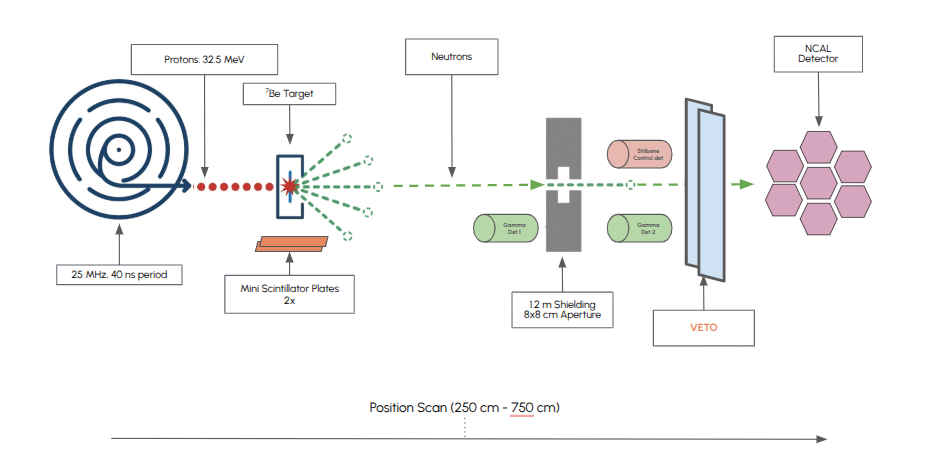
\includegraphics[width=0.98\textwidth]{figures/Experiment_Setup_rez2.png}
\caption{Schematic layout of the second experiment at \NCALInstitute. The scheme shows the proton beam delivered from the cyclotron onto a beryllium target, target-adjacent mini scintillator plates planned as a coincidence-based backup production monitor, an upstream gamma detector, a \SI{1.2}{m} shielding block with an $8 \times 8$ cm$^2$ aperture aligned to the central NCAL line of sight, a downstream gamma detector behind the shield, a compact control stilbene detector near the NCAL entrance plane, the seven-module NCAL flower geometry, and an optional thin plastic veto layer in front of the central module. The position-scan direction indicated in the sketch corresponds to the current working range of roughly \SIrange{250}{750}{cm}. Several elements, especially the target-adjacent scintillators, the exact control-detector placement, and the use of the front veto layer, remained part of the ongoing setup optimization.}
\label{fig:rez2-working-setup}
\end{figure}

The experiment was performed in the forward-directed mixed neutron--gamma field produced by cyclotron protons on a beryllium target. The forward radiation field emerging from the target was sampled downstream along the axis of the planned NCAL position scan. The drawing presently labels the proton beam with an energy of \SI{32.5}{MeV} and also marks the cyclotron RF structure as \SI{25}{MHz} with a \SI{40}{ns} period. These values are retained here as setup identifiers from the current experiment sketch and should be cross-checked against the run-time machine settings recorded during the actual campaign.

One distinctive feature of the planned geometry is the pair of mini scintillator plates placed immediately next to the target and oriented toward the production point. In the present concept they are intended to operate in coincidence mode and to provide a local indication that production is taking place near the target. Their role is explicitly secondary: they are currently treated as a backup or plan-B monitoring option rather than as a validated primary beam monitor. Their efficiency in the actual source geometry, their count-rate capability, and even their practical usefulness under the expected radiation conditions are not yet established and will need to be tested experimentally.

Farther downstream, the first gamma detector is intended to monitor the prompt and background gamma field before the main shielding block. The present expectation is that this detector may provide both gamma-spectral information and useful timing information associated with prompt gamma production. A \SI{1.2}{m} thick shielding block with an $8 \times 8$ cm$^2$ aperture is then used to define the line of sight toward the central NCAL module. In the current layout logic, the aperture is not merely a mechanical opening but part of the background-reduction strategy: it restricts the direct acceptance to the intended central region while allowing the surrounding shield to suppress off-axis radiation.

Behind this shielding block, a second gamma detector is planned upstream of NCAL but in a substantially more shielded location than the first one. Its intended role is to characterize the radiation field that survives the shielding and reaches the NCAL entrance region. In the most conservative wording, this means measuring the gamma spectrum behind the shielding; depending on detector response and local mixed-field conditions, the same detector may also record neutron-induced contributions, but that possibility should be treated as an effect to be measured rather than assumed a priori.

The control stilbene detector is presently envisaged near the NCAL entrance plane as a reference neutron monitor with known neutron-detection performance. Its exact position, however, remains an open optimization problem. From one point of view, the most direct comparison would place it on the same central line of sight as the central NCAL module. From another point of view, material placed directly in front of NCAL may partially shadow the calorimeter acceptance or generate additional secondary particles. For that reason, the final measurement sequence may need to alternate between different control-detector positions, or between control-detector and unobstructed NCAL configurations, instead of assuming a single permanent placement from the outset.

The NCAL detector itself is planned in the seven-module flower arrangement consisting of one central module surrounded by six peripheral modules in a honeycomb-like hexagonal pattern. The central module is aligned with the shielding aperture and therefore defines the primary line of interest in the present setup concept. In addition, a thin plastic scintillator layer may be placed in front of the central module as a veto for charged particles. At present this veto layer should be regarded as a diagnostic option rather than an established component of the finalized setup. The current expectation from the local beamline side is that charged particles should not emerge from the target region in a way that significantly reaches the NCAL position, but this statement still requires direct confirmation under the actual experimental conditions.

\section{Experimental subsystems and their roles}

Although the NCAL prototype is the detector under study, the full experiment involves several coupled subsystems. Their roles are summarized in Table~\ref{tab:experiment-subsystems}. This distinction is important because later chapters discuss some of these elements separately in terms of hardware documentation, but at experiment level they function together as one measurement system.

\begin{table}[htbp]
\centering
\caption{Main experimental subsystems and their role in the present campaign.}
\label{tab:experiment-subsystems}
\small
\setlength{\tabcolsep}{5pt}
\renewcommand{\arraystretch}{1.08}
\begin{tabularx}{\textwidth}{>{\raggedright\arraybackslash}p{3.5cm}YY}
\toprule
Subsystem & Role in the experiment & Main observables or function \\
\midrule
NCAL prototype & Detector under study & Neutron response, timing behavior, detector stability, and future efficiency-related observables \citep{Okropiridze2024SimulationNCAL,Okropiridze2026NCALAddendum}. \\
Target-adjacent mini scintillator pair (planned) & Backup production monitor near the target & Local coincidence signal near the production point; presently a contingency monitor whose practical efficiency is not yet established. \\
First gamma detector & Upstream mixed-field monitor & Prompt-gamma timing information and gamma-spectrum monitoring before the main shielding block. \\
Shielding block with central aperture & Passive background reduction and geometrical selection & Restricts the direct line of sight toward the central NCAL module while suppressing off-axis radiation. \\
Second gamma detector & Downstream radiation-field monitor & Characterization of the radiation field behind shielding and in front of NCAL, primarily gamma-sensitive but potentially recording mixed-field contributions. \\
Control stilbene detector & Reference neutron monitor & Relative neutron-flux monitoring close to the NCAL entrance region, with placement still under optimization. \\
Optional thin plastic veto layer & Charged-particle check at the NCAL entrance plane & Diagnostic veto option intended to test whether any charged-particle contamination reaches the calorimeter position. \\
DAQ and front-end chains & Signal transport and event building & Trigger-referenced observables such as timestamps, time-over-threshold values, timing jitter, waveform shapes, and firmware-derived quantities. \\
\bottomrule
\end{tabularx}
\end{table}

The upstream and downstream gamma detectors, the control stilbene detector, and the target-adjacent mini scintillators each probe a different part of the radiation field and together provide the contextual information needed to interpret the NCAL response. The shielding and aperture assembly likewise form an active part of the measurement definition, because they determine which fraction of the field is intentionally delivered to the calorimeter entrance.

\section{Measurement strategy}

The measurement strategy is centered on the NCAL flower geometry aligned to the shielding aperture and studied along the beam axis over the planned source-to-detector distance range indicated in Fig.~\ref{fig:rez2-working-setup}. Supporting detectors are used to characterize different components of the local radiation field: the upstream gamma detector samples the prompt field before shielding, the downstream gamma detector characterizes the radiation that reaches the NCAL entrance region, and the control stilbene detector provides a neutron-sensitive reference close to the calorimeter position.

Additional configuration changes remain part of the experimental strategy where required by the measurement conditions. In particular, the exact placement of the control stilbene detector may be alternated to avoid permanent shadowing of the central NCAL line of sight, and the thin plastic veto layer may be inserted as a diagnostic configuration to test for any charged-particle contribution at the calorimeter entrance. Within this framework, the later analysis can focus on direct NCAL observables together with the contextual timing and background information delivered by the supporting detector chains.
\chapter{Production Physics}

\section{Beryllium-target neutron production at NPI}

For the present NCAL campaign, the relevant source environment is the proton-driven neutron production line operated at the U-120M cyclotron at NPI \v{R}e\v{z}. The source literature available in this workspace shows that two related, but physically distinct, beryllium-based configurations are used there and should not be conflated. In the thick-target configuration, \SI{35}{MeV} protons are fully stopped in an \SI{8}{mm} beryllium target and produce a continuous fast-neutron spectrum extending up to about \SI{33}{MeV} \citep{Majerle2023PBeGenerator}. In the collimated-beam configuration, protons interact with a \SI{2.5}{mm} beryllium foil, lose only part of their energy in the beryllium, and are then stopped downstream in a carbon slab; in that case the forward spectrum retains a quasi-monoenergetic character \citep{Ansorge2025CollimatedBeams}.

This distinction matters for any discussion of the accompanying gamma field. A statement such as ``gamma spectrum for \SI{35}{MeV} protons on thick Be'' is incomplete unless the surrounding station geometry is also specified. The gamma background depends not only on the primary proton--beryllium interaction, but also on which additional beamline elements are struck by the proton beam and which materials are present close to the source.

The neutron-production papers also show that some structures in the forward spectrum arise from different \(^{9}\mathrm{Be}(p,n)\) channels feeding the ground and low-lying excited states of \(^{9}\mathrm{B}\) \citep{Ansorge2025CollimatedBeams,Majerle2023PBeGenerator}. These structures are neutron-spectrum features. They should not be reinterpreted as evidence for prominent prompt gamma lines from \(^{9}\mathrm{B}^{*}\) de-excitation.

\section{Dominant neutron-production channels}

The reviewed NPI source papers support a compact interpretation of the forward neutron spectrum at proton energies around \SI{35}{MeV}. Thin-target measurements cited in these works show two high-energy components associated with the \(^{9}\mathrm{Be}(p,n)\) charge-exchange reaction, corresponding to population of the ground state of \(^{9}\mathrm{B}\) and of its first two excited states at \SI{2345}{keV} and \SI{2751}{keV}, superimposed on a broader continuum from compound-nucleus reactions \citep{Majerle2023PBeGenerator,Ansorge2025CollimatedBeams}. In the thick-target configuration, the measured forward spectrum is then interpreted as the superposition of such partial spectra as the incident protons slow down in the beryllium. This produces the characteristic step-like structure observed near \SIrange{30}{32}{MeV} \citep{Majerle2023PBeGenerator}.

\begin{table}[htbp]
\centering
\caption{Source-supported neutron-production channels relevant for the forward spectrum from \SI{35}{MeV} protons on a thick beryllium target.}
\begin{tabular}{p{3.8cm}p{3.1cm}p{5.7cm}}
\toprule
Channel & Spectral manifestation & Comment \\
\midrule
\(^{9}\mathrm{Be}(p,n){}^{9}\mathrm{B}_{\mathrm{g.s.}}\) & Highest-energy component, extending to about \SI{33}{MeV} & Forms the upper part of the high-energy peak structure in the forward spectrum \citep{Majerle2023PBeGenerator}. \\
\(^{9}\mathrm{Be}(p,n){}^{9}\mathrm{B}^{*}\) to the first two excited states at \SIlist{2345;2751}{keV} & Second component about \SI{2.5}{MeV} lower than the highest peak & Together with the ground-state channel it produces the step-like structure near \SIrange{30}{32}{MeV}. The literature cited by Majerle et al. indicates an approximate 6:4 area ratio between the upper and lower high-energy components \citep{Majerle2023PBeGenerator}. \\
Compound-nucleus contribution & Broad continuum underlying the peaks and extending to lower neutron energies & Described explicitly in the NPI beam papers as the continuum component of the spectrum \citep{Majerle2023PBeGenerator,Ansorge2025CollimatedBeams}. \\
\bottomrule
\end{tabular}
\end{table}

The same thick-target study also shows that very close to the source the measured spectrum is modified by scattering in the target-station construction materials and by the finite extent of the production region. For that specific NPI configuration, Monte Carlo simulations indicate that this effect becomes negligible by about \SI{50}{cm} from the beryllium slab, after which inverse-square scaling is used for the flux normalization \citep{Majerle2023PBeGenerator}. For scan distances of order \SIrange{2.5}{7.5}{m}, this supports the use of \(1/r^{2}\) as a first-order geometric scaling law, provided the same source-station configuration is maintained.

\section{Expected gamma contributions}

Only a limited set of gamma contributions can be stated with confidence from the presently available beamline literature. Since the gamma field depends on the exact source-station geometry, beam centering, and the distribution of carbon- and hydrogen-containing materials near the target, a detailed line-by-line intensity model is not introduced here. Instead, only source terms directly supported by the reviewed NPI references are summarized.

The best established prompt contribution is the \SI{4.439}{MeV} line from excited \(^{12}\mathrm{C}\). In the collimated-beam study, the prompt gamma timing peak is attributed to proton-beam interaction with the carbon stopping slab and the subsequent de-excitation of \(^{12}\mathrm{C}\), explicitly identifying the \SI{4439}{keV} transition \citep{Ansorge2025CollimatedBeams}. In the thick-target neutron-generator study, prompt gamma peaks are likewise associated with proton-beam interaction with a carbon beam collimator located upstream of the beryllium target \citep{Majerle2023PBeGenerator}. A prompt carbon line near \SI{4.44}{MeV} is therefore a realistic expectation whenever carbon components in the source station intercept part of the proton beam.

The same collimated-beam study also discusses the \SI{2224}{keV} gamma from the \(^{1}\mathrm{H}(n,\gamma)\) reaction \citep{Ansorge2025CollimatedBeams}. This line is relevant for the local radiation environment and detector response, but it should be interpreted as a secondary environmental gamma from neutron capture in hydrogenous material rather than as a primary prompt component of proton--beryllium production.

The available references do not justify fixed yield fractions for individual gamma lines, and they do not provide sufficient support for a detailed source decomposition involving additional discrete lines or a dominant continuum component for the present geometry. Those features should therefore be introduced only after dedicated gamma spectroscopy or transport calculations for the finalized setup.

\begin{table}[htbp]
\centering
\caption{Working expectations for gamma contributions relevant to beryllium-target operation at NPI \v{R}e\v{z}.}
\begin{tabular}{p{3.3cm}p{3.3cm}p{6.0cm}}
\toprule
Source region & Signature & Comment \\
\midrule
Carbon beamline components & Prompt line near \SI{4.439}{MeV} & Supported when the proton beam intercepts carbon elements such as the beam collimator or carbon stopping slab \citep{Ansorge2025CollimatedBeams,Majerle2023PBeGenerator}. \\
Hydrogenous material near the source or detector & Secondary line at \SI{2.224}{MeV} & Associated with \(^{1}\mathrm{H}(n,\gamma){}^{2}\mathrm{H}\); relevant for environmental background and calibration-related response \citep{Ansorge2025CollimatedBeams}. \\
Other prompt components & Geometry dependent & Additional lines or continuum components should not be quantified without a run-specific measurement or transport simulation. \\
\bottomrule
\end{tabular}
\end{table}

\section{Implications for the NCAL analysis}

For the present NCAL document, the safest working assumption is therefore a limited one: the prompt-gamma field should be expected to contain at least a strong timing component associated with fast source gammas, and a \SI{4.439}{MeV} carbon line is physically plausible whenever carbon beamline components are irradiated. Beyond that, the detailed line content and relative intensities should be considered geometry-dependent and not fixed a priori. In particular, if the actual run conditions differ from the \SI{35}{MeV} reference papers in proton energy, beam centering, source hardware, shielding composition, or aperture arrangement, then the gamma spectrum must be re-evaluated for the exact run geometry rather than copied from a generic source table.

Accordingly, the present document treats the gamma spectrum only at the level justified by currently available evidence. Any quantitative spectral decomposition should be based on either a dedicated gamma measurement with an energy-calibrated detector or a transport calculation using the finalized source-station geometry and realistic material composition. Until such a study is completed, the table above should be regarded as a compact working expectation rather than a final spectral model.
\chapter{Experimental Detector Systems}

This chapter summarizes the detector systems currently used in the experiment and the parts of their readout chains that matter for operation and data interpretation. The present hardware inventory includes a primary gamma-spectroscopy detector, consisting of an ORTEC 905-4 NaI(Tl) detector head coupled to an ORTEC Model 276 photomultiplier base with integrated preamplifier, two auxiliary thin scintillation counters instrumented with compact Hamamatsu PMT hardware, and one compact stilbene-based parallel monitor detector provided by the beamline team at \NCALInstitute. The discussion is organized by detector system rather than by vendor component alone, because in practical operation the experimentally relevant object is the full detector-plus-readout chain.

\section{Detector inventory and intended role}

Table~\ref{tab:detector-summary} summarizes the detector systems presently identified for the campaign in a compact form suitable for later comparison of detector medium, sensor chain, biasing, signal compatibility, and experimental role. Where a parameter has not yet been verified directly in the available documentation or campaign notes, it is marked explicitly as not yet verified rather than inferred.

\begin{landscape}
\begin{table}[p]
\centering
\caption{Summary of detector systems presently identified for the campaign.}
\label{tab:detector-summary}
\small
\setlength{\tabcolsep}{3.5pt}
\renewcommand{\arraystretch}{1.12}
\begin{tabularx}{\linewidth}{>{\raggedright\arraybackslash}p{2.3cm}>{\raggedright\arraybackslash}p{2.6cm}>{\raggedright\arraybackslash}p{3.1cm}>{\centering\arraybackslash}p{0.9cm}>{\raggedright\arraybackslash}p{2.4cm}>{\raggedright\arraybackslash}X>{\raggedright\arraybackslash}p{2.2cm}Y}
\toprule
Detector & \shortstack[c]{Detector\\medium} & \shortstack[c]{Sensor /\\Readout} & \multicolumn{1}{c}{Qty} & \shortstack[c]{HV\\range} & \shortstack[c]{Signal\\range} & \shortstack[c]{Signal\\polarity} & Role \\
\midrule
ORTEC 905-4 chain & 3-inch $\times$ 3-inch NaI(Tl) crystal & 3-inch PMT + ORTEC 276 base/preamplifier & 1 & Positive HV up to \SI{2000}{V} at the base & Branch dependent; preamp and anode outputs serve different purposes & Positive preamp output; negative anode output & Gamma spectroscopy; calibration; threshold studies; commissioning support \\
Thin plastic scintillation counters & Thin plastic detectors; dimensions N/A & Hamamatsu E1761-04 socket assembly for 10 mm PMTs & 2 & Negative HV up to \SI{1500}{V} & Setup-specific pulse amplitude not yet verified in archived notes & Negative & Charged-particle or prompt-timing support; coincidence studies; auxiliary trigger work \\
SCIONIX stilbene monitor & 5 $\times$ 5 $\times$ 15 mm crystalline stilbene & Hamamatsu R12421 PMT, direct raw-anode readout & 1 & Negative HV in assembled probe; PMT $|V_{\mathrm{AK}}|$ up to \SI{1250}{V} & Several-hundred-ns negative anode pulses; typically few-hundred-mV into \SI{50}{\ohm}, possibly approaching about \SI{1}{V} in current working notes & Negative & Parallel neutron monitor and relative beam-flux reference \\
\bottomrule
\end{tabularx}
\par\smallskip
\begin{minipage}{\linewidth}
\footnotesize
\textit{Sources:} Gamma-detector entry compiled from the ORTEC 905-series detector documentation and the ORTEC Model 276 manual \citep{ORTEC905SeriesManual,ORTEC276Manual}. Thin-plastic-detector readout and high-voltage limits from the Hamamatsu E1761-04 documentation \citep{HamamatsuE176104Page}. Stilbene-monitor PMT and high-voltage limits from the Hamamatsu R12421 datasheet \citep{HamamatsuR12421Manual}; assembly identification and setup-specific signal working values from current campaign notes.
\end{minipage}
\end{table}
\end{landscape}

\section{Primary gamma-spectroscopy detector chain}

The primary detector chain for the auxiliary gamma-ray measurements and calibration studies is a conventional scintillation assembly composed of an ORTEC 905-4 NaI(Tl) detector head and an ORTEC Model 276 photomultiplier base with integrated preamplifier. In the local hardware inventory, the detector head is additionally identified as an Alpha Spectra, Inc. model 12I12/3. These two components should be treated as a single measurement chain: the NaI(Tl) crystal converts deposited gamma-ray energy into scintillation light, the photomultiplier tube (PMT) converts that light into charge, and the Model 276 base supplies both the dynode bias distribution and the first analog conditioning stage \citep{ORTEC905SeriesManual,ORTEC276Manual}.

\subsection{ORTEC 905-4 NaI(Tl) detector head}

The ORTEC 905 series is a family of NaI(Tl) scintillation detectors intended primarily for gamma-ray counting and spectroscopy \citep{ORTEC905SeriesManual}. For the present work, the relevant unit is the 905-4 configuration, which combines a 3-inch diameter by 3-inch long NaI(Tl) crystal with a 3-inch PMT. This geometry is a standard compromise between absolute efficiency, moderate intrinsic energy resolution, and mechanical simplicity. Because iodine has a relatively high atomic number, NaI(Tl) retains a comparatively large full-energy absorption probability for laboratory gamma sources, which is one reason why this detector class remains a practical choice for commissioning, calibration, and source-based verification.

The 905-series datasheet emphasizes the standard physical advantages and limitations of NaI(Tl) detectors \citep{ORTEC905SeriesManual}. Their light output is sufficiently large for routine spectroscopy, and the manufacturer quotes a typical resolution of about 7\% at $^{137}$Cs for a 3-inch by 3-inch crystal, with somewhat worse values for larger detectors. At the same time, NaI(Tl) is not a particularly fast scintillator: the light decay constant is about \SI{0.23}{\micro\second}, and with a typical charge-sensitive front end this corresponds to an output-voltage rise time of about \SI{0.5}{\micro\second}. Consequently, the detector is well suited to efficiency-oriented gamma counting and moderate-resolution energy measurements, but it is not the natural choice when the best possible sub-nanosecond timing performance is required.

For the present report, two practical remarks from the manufacturer documentation are especially relevant. First, the 905-series detector heads are supplied to ORTEC by specialized detector manufacturers, so minor parameter differences between nominally identical detector heads are possible \citep{ORTEC905SeriesManual}. Second, the datasheet quotes representative total counting efficiencies for a $1$-$\mu$Ci $^{137}$Cs source positioned at a distance of \SI{10}{cm}; these values are useful as order-of-magnitude expectations during laboratory checkout, but they should not be mistaken for a substitute for an experiment-specific efficiency calibration.

\begin{table}[htbp]
\centering
\caption{Manufacturer information most relevant to the ORTEC 905-4 detector used in the present setup.}
\label{tab:ortec9054-specs}
\small
\setlength{\tabcolsep}{5pt}
\renewcommand{\arraystretch}{1.08}
\begin{tabularx}{\textwidth}{>{\raggedright\arraybackslash}p{4.2cm}YY}
\toprule
Parameter & Value & Comment \\
\midrule
Detector family & ORTEC 905 series NaI(Tl) scintillation detector & Modular scintillation-detector family for gamma-ray measurements \citep{ORTEC905SeriesManual}. \\
Nominal detector size & 3-inch diameter $\times$ 3-inch length crystal & ORTEC model 905-4; the local assembly is identified as Alpha Spectra model 12I12/3. \\
Photomultiplier size & 3-inch PMT & Integral part of the detector head supplied with the 905-4 configuration \citep{ORTEC905SeriesManual}. \\
Typical energy resolution & About 7\% at $^{137}$Cs for a 3-inch by 3-inch crystal & Representative manufacturer value for routine gamma spectroscopy. \\
Light decay constant & About \SI{0.23}{\micro\second} & Sets a lower bound on the detector pulse width and therefore influences timing performance. \\
Typical voltage-pulse rise time & About \SI{0.5}{\micro\second} with a typical charge-sensitive preamplifier & Useful for estimating shaping or record-length requirements in downstream electronics. \\
Typical total counting efficiency & 2.00\% at \SI{0.5}{MeV} and 1.30\% at \SI{2.0}{MeV} for a $1$-$\mu$Ci $^{137}$Cs source at \SI{10}{cm} & Quoted specifically for the 905-4 geometry; intended as a comparative detector figure rather than an in-beam calibration. \\
\bottomrule
\end{tabularx}
\end{table}

\subsection{ORTEC Model 276 photomultiplier base with integrated preamplifier}

The ORTEC Model 276 is not merely a passive PMT socket. It is a combined PMT base and analog front-end designed for essentially all 10-stage photomultipliers that fit the standard 14-pin socket geometry \citep{ORTEC276Manual}. The instrument contains a resistor-divider bleeder chain for dynode biasing, a focus adjustment for optimizing the photocathode-to-first-dynode field, an ac-coupled anode output intended mainly for timing applications, and a self-contained low-noise integrating preamplifier coupled to the last dynode for spectroscopy-oriented energy readout \citep{ORTEC276Manual}. In practical terms, the device therefore separates the detector signal into two complementary observables: a fast negative anode pulse for timing work and a slower positive preamplifier pulse for energy analysis.

The manufacturer specifications show why the Model 276 is suitable for routine scintillation spectroscopy. The PMT divider has a total resistance of \SI{1.49}{\mega\ohm} and draws about \SI{1.33}{mA} at the maximum applied voltage of \SI{2000}{V}. The integrated preamplifier has a nominal conversion gain of \SI{5}{\micro\volt\per\electronvolt} for a reference configuration consisting of a 2-inch by 2-inch NaI(Tl) crystal and a PMT gain of $10^{6}$; the same manual quotes a rise time below \SI{100}{ns} for a fast test pulse, a fall-time constant of \SI{50}{\micro\second}, and an output noise below \SI{50}{\micro\volt} rms \citep{ORTEC276Manual}. These numbers should be interpreted as front-end performance parameters rather than as immutable detector properties, because the actual pulse amplitude still depends on the detector head, the PMT installed, and the chosen high-voltage operating point.

The Model 276 manual also provides the key operational constraints relevant to the present work. The PMT base expects a positive high-voltage supply with a maximum value of \SI{2000}{V}, the detector--PMT assembly must be made fully light-tight, and the single-turn focus potentiometer must be adjusted under irradiation so that the pulse amplitude is maximized and then mechanically locked \citep{ORTEC276Manual}. The manual further notes that the photomultiplier gain changes by approximately a factor of two for each \SI{100}{V} change in high voltage, so the actual gain setting is highly sensitive to the chosen bias voltage.

\begin{table}[htbp]
\centering
\caption{Selected specifications of the ORTEC Model 276 relevant to detector operation and DAQ coupling.}
\label{tab:ortec276-specs}
\small
\setlength{\tabcolsep}{5pt}
\renewcommand{\arraystretch}{1.08}
\begin{tabularx}{\textwidth}{>{\raggedright\arraybackslash}p{4.2cm}YY}
\toprule
Parameter & Value & Comment \\
\midrule
PMT compatibility & Standard 14-pin, 10-stage photomultipliers & Designed to provide near-optimum voltage distribution for this PMT class \citep{ORTEC276Manual}. \\
Maximum high voltage & Positive \SI{2000}{V} & The supply polarity is positive, with the cathode at ground potential. \\
Divider resistance & \SI{1.49}{\mega\ohm} total bleeder resistance & Corresponds to a bleeder current of about \SI{1.33}{mA} at \SI{2000}{V}. \\
Focus adjustment & External single-turn locking potentiometer & Used to optimize the photocathode-to-first-dynode field under operating conditions. \\
Preamplifier output & Positive, dc-coupled energy-analysis signal & Intended primarily for spectroscopy-oriented acquisition. \\
Anode output & Negative, ac-coupled pulse & Intended primarily for timing and coincidence work. \\
Nominal preamplifier conversion gain & \SI{5}{\micro\volt\per\electronvolt} in the reference 2-inch by 2-inch NaI(Tl) configuration & Reference value only; the actual output depends on detector, PMT, and high voltage. \\
Preamplifier rise time & $<\SI{100}{ns}$ for a fast test pulse & Indicates that the base itself does not dominate the slower NaI(Tl) scintillation time scale. \\
Preamplifier fall-time constant & \SI{50}{\micro\second} & Relevant for shaping and pile-up considerations at higher count rates. \\
Output noise & $<\SI{50}{\micro\volt}$ rms & Useful lower bound when evaluating baseline quality. \\
Power requirements & $+\SI{24}{V}$ at \SI{16}{mA} and $-\SI{24}{V}$ at \SI{16}{mA} & Compatible with ORTEC main amplifiers or the ORTEC 114 preamplifier power supply \citep{ORTEC276Manual}. \\
\bottomrule
\end{tabularx}
\end{table}

\subsection{Operational settings relevant to the ORTEC NaI(Tl) chain}

For the present NCAL-related laboratory work, the most important result of the manufacturer documentation is that there is no single universal bias setting that can be adopted blindly. The recommended procedure is instead operational: the detector must first be made light-tight, a positive high-voltage supply is then connected, and the high voltage is increased slowly while the preamplifier output is observed in the presence of a radiation source \citep{ORTEC276Manual}. If a large amount of unipolar ``grass'' appears on the oscilloscope trace, the manual recommends checking explicitly for a light leak by covering the PMT region with an opaque cloth. Only after the detector has been verified to be optically sealed should the operating voltage be optimized.

The focus control is the second essential setting. According to the Model 276 manual, the correct procedure is to set the high voltage near the desired operating level, observe radiation-induced pulses, adjust the focus for maximum pulse amplitude, and then lock the potentiometer mechanically \citep{ORTEC276Manual}. This is a physically meaningful adjustment rather than a cosmetic one, because it optimizes electron collection from the photocathode to the first dynode and therefore influences both gain stability and pulse-height response.

For routine acquisition, the manufacturer explicitly advises using the minimum practical high voltage when high count rates are expected, because count-rate tolerance is directly connected to the PMT gain and the gain changes by roughly a factor of two per \SI{100}{V} \citep{ORTEC276Manual}. In the context of a digitizer-based DAQ chain, this has two immediate consequences. First, the applied bias voltage should be documented together with each accepted configuration, because modest voltage changes can shift the effective gain substantially. Second, the digitizer settings must match the signal branch that is actually digitized: the preamplifier output is the natural branch for energy analysis and has positive polarity, whereas the anode output is the natural branch for timing studies and has negative polarity. A threshold or polarity configuration validated on one branch should therefore not be transferred to the other without re-optimization.

The manual also offers a simple functional calibration check that is useful during bench setup: a \SI{1}{V} test pulse injected into the TEST input should yield a \SI{1}{V} pulse at the preamplifier output \citep{ORTEC276Manual}. This provides a straightforward verification that the base, preamplifier power, and downstream readout chain are behaving consistently before radioactive-source measurements are attempted.

Taken together, the ORTEC 905-4 and the ORTEC 276 form a robust, conventional scintillation-detector chain for laboratory gamma spectroscopy and detector commissioning. The detector head offers the expected efficiency advantages of a 3-inch by 3-inch NaI(Tl) crystal, while the base and preamplifier provide the biasing, gain control, and signal extraction needed to couple the assembly to either classical NIM electronics or a modern waveform digitizer. For the present campaign, these characteristics make the system well suited to calibration runs, threshold studies, and first-response checks of the broader NCAL readout infrastructure.

\section{Auxiliary thin plastic detectors}

The setup also includes two thin plastic detectors used as auxiliary counters. The presently available hardware identification for their optical readout is the Hamamatsu E1761-04 D-type socket assembly, which Hamamatsu specifies for 10~mm diameter head-on photomultiplier tubes \citep{HamamatsuE176104Page}. This places the readout in the class of compact PMT assemblies rather than large-area spectroscopy bases. In practical detector terms, that geometry is well matched to lightweight auxiliary detectors, where compactness and prompt signal pickup are more important than the absolute full-energy efficiency expected from a much larger NaI(Tl) head.

The manufacturer specification most relevant to detector operation is electrical rather than mechanical. Hamamatsu lists the E1761-04 with negative high-voltage polarity, a maximum supply voltage of \SI{1500}{V}, and the same \SI{1500}{V} maximum rating between the case and connector pins \citep{HamamatsuE176104Page}. The integrated voltage-divider chain has a total resistance of \SI{3.63}{\mega\ohm}, corresponding to a maximum divider current of \SI{0.41}{mA} at the rated voltage. The product page further quotes a maximum leakage current of $1.0\times10^{-10}$~A at the signal output and a maximum linear dc output current of \SI{20}{\micro A} at \SI{1500}{V} \citep{HamamatsuE176104Page}. Current setup notes additionally identify the readout polarity used for these detectors as negative. Taken together, these are the main verified limits and operating characteristics that matter when the counters are connected to external high voltage, discriminators, or digitizer inputs.

At present, the local notes establish the detector bodies as thin plastic detectors mounted with Hamamatsu E1761-04 assemblies. The exact scintillator trade name, active area, and thickness are not yet verified from manufacturer documentation available in the workspace. Rather than introducing unsupported dimensions or assigning a plastic formulation that is not documented locally, Table~\ref{tab:hamamatsu-e1761-04-specs} records the verified detector-type and readout specifications and leaves the remaining body parameters to be added later, once the counters are measured directly or their original labels are recovered.

\begin{table}[htbp]
\centering
\caption{Verified readout specifications for each of the two auxiliary thin scintillation counters equipped with Hamamatsu E1761-04 hardware.}
\label{tab:hamamatsu-e1761-04-specs}
\small
\setlength{\tabcolsep}{5pt}
\renewcommand{\arraystretch}{1.08}
\begin{tabularx}{\textwidth}{>{\raggedright\arraybackslash}p{4.2cm}YY}
\toprule
Parameter & Value & Comment \\
\midrule
Number of counters in setup & 2 & Pair of auxiliary thin scintillation counters planned for the present campaign. \\
Detector-body type & Thin plastic detector & Established in current setup notes; exact plastic grade and dimensions remain unverified. \\
Readout assembly & Hamamatsu E1761-04 D-type socket assembly & Manufacturer-designated PMT socket assembly used on the counters \citep{HamamatsuE176104Page}. \\
Applicable PMT & 10~mm head-on type & Hamamatsu specification for the E1761-04 assembly. \\
Readout signal polarity & Negative & Current setup notes identify negative signal polarity for these counters. \\
Supply voltage polarity & Negative & The assembly is intended for negative high-voltage operation. \\
Maximum supply voltage & \SI{1500}{V} & Manufacturer maximum rating for operation. \\
Maximum insulation voltage (case to pins) & \SI{1500}{V} & Important when integrating the assembly into grounded mechanical supports. \\
Total voltage-divider resistance & \SI{3.63}{\mega\ohm} & Sets the divider current and power dissipation at the chosen operating voltage. \\
Maximum voltage-divider current & \SI{0.41}{mA} & Quoted at rated voltage by Hamamatsu. \\
Maximum leakage current in signal output & $1.0\times10^{-10}$~A & Upper bound from the product specification. \\
Maximum linear dc output current & \SI{20}{\micro A} at \SI{1500}{V} & Useful when estimating acceptable load conditions. \\
Exact plastic grade / dimensions presently verified & Not yet identified & Active area, thickness, and scintillator trade name should be added after direct inspection of the two counters. \\
\bottomrule
\end{tabularx}
\end{table}

\section{Facility-provided parallel stilbene monitor}

In addition to the detector systems brought by the NCAL group, the beamline team at \NCALInstitute indicated that one compact stilbene-based monitor detector would be operated in parallel with the NCAL measurements as an online flux reference. In the available campaign coordination notes, this detector is identified as a SCIONIX model \texttt{V5B15/0.5-E1-STILB-X-NEG}, consisting of a 5 $\times$ 5 $\times$ 15 mm stilbene crystal optically coupled to a Hamamatsu \texttt{R12421} photomultiplier tube. A dedicated public datasheet for this exact assembled probe is not presently archived in the workspace. The description below therefore separates three layers of information that should not be conflated: assembly-level identification from campaign notes, material-level properties of crystalline stilbene from vendor documentation, and tube-level characteristics of the Hamamatsu photomultiplier from its manufacturer datasheet.

As a detector medium, stilbene belongs to the class of hydrogen-rich organic scintillators used for fast-neutron detection. Scionix summarizes the basic detection logic by noting that fast neutrons are detected in organic scintillators mainly through recoil protons, and that neutron--gamma separation is possible by pulse-shape discrimination when neutron and gamma interactions lead to different scintillation decay behavior \citep{ScionixNeutronScintillatorNote}. The Inrad application note describes crystalline stilbene as particularly suitable for fast-neutron identification in the presence of gamma background and lists a density of \SI{1.15}{\gram\per\centi\meter\cubed}, a maximum emission wavelength of about \SI{380}{nm}, a prompt decay time of about \SI{4.3}{ns}, and a rise time of about \SI{0.1}{ns} \citep{InradStilbeneNote}. These are material-level quantities rather than guaranteed performance numbers for the specific SCIONIX assembly used here, but they explain why stilbene is a scientifically reasonable choice for a compact reference detector in a mixed neutron--gamma field.

The same stilbene note describes neutron--gamma separation in terms of different prompt and delayed fluorescence fractions and presents vendor data with a pulse-shape-discrimination figure of merit of 4.7 near \SI{500}{keVee}, with separation demonstrated down to \SI{22}{keVee} and reported gamma misclassification rates of $10^{-6}$ \citep{InradStilbeneNote}. For the present report, however, those figures should be treated only as indicative literature-level performance for high-quality stilbene and an optimized PSD chain. They should not be promoted to established performance of the particular 5 $\times$ 5 $\times$ 15 mm control detector unless the assembled probe is characterized directly under the same acquisition conditions used in the campaign.

At the photosensor level, Hamamatsu specifies the R12421 as a compact 13 mm diameter photomultiplier tube with a 10 mm effective area, a bialkali photocathode, 10 dynode stages, a spectral response from 300 to 650 nm, and a peak response near \SI{420}{nm} \citep{HamamatsuR12421Manual}. The same datasheet gives a typical gain of $2.0\times10^{6}$ at \SI{1000}{V}, an anode pulse rise time of about \SI{1.2}{ns}, and a maximum anode-to-cathode voltage magnitude of \SI{1250}{V} \citep{HamamatsuR12421Manual}. This spectral response is technically compatible with stilbene emission in the blue-violet region, so the R12421 is a consistent readout choice for a compact stilbene monitor operated without an intermediate wavelength-shifting stage.

For the present campaign, current working notes indicate direct raw-anode readout with negative polarity and negative high-voltage operation of the assembled detector. The working pulses are described as several hundred nanoseconds wide and typically in the few-hundred-mV range into \SI{50}{\ohm}, with amplitudes potentially approaching about \SI{1}{V} at operating bias. Because the factory sheet for the exact SCIONIX assembly is not yet available locally, these signal-level statements should be interpreted as setup-specific working values rather than universal device specifications.

The most defensible experimental role of this detector in the present setup is therefore that of a relative neutron monitor and beam-reference channel. The crystal is intentionally compact, and the Scionix detector note explicitly remarks that efficient fast-neutron detection requires a significant absorption volume \citep{ScionixNeutronScintillatorNote}. Accordingly, the probe is well suited to tracking relative beam conditions and providing a compact PSD-capable reference detector in parallel with the main NCAL measurement, but it should not be treated in this report as an absolutely calibrated neutron-efficiency instrument unless a separate dedicated calibration is performed.

\begin{table}[htbp]
\centering
\caption{Selected characteristics of the facility-provided stilbene monitor.}
\label{tab:scionix-stilbene-specs}
\footnotesize
\setlength{\tabcolsep}{4pt}
\renewcommand{\arraystretch}{1.02}
\begin{tabularx}{\textwidth}{>{\raggedright\arraybackslash}p{3.8cm}YY}
\toprule
Parameter & Value & Comment \\
\midrule
Assembly identifier & SCIONIX \texttt{V5B15/0.5-E1-STILB-X-NEG} & Control-detector identification from campaign notes. \\
Scintillator material & Crystalline stilbene & PSD-capable organic fast-neutron scintillator \citep{InradStilbeneNote,ScionixNeutronScintillatorNote}. \\
Nominal crystal size & 5 $\times$ 5 $\times$ 15 mm & Size recorded for the assembled probe in campaign notes. \\
Stilbene density & \SI{1.15}{\gram\per\centi\meter\cubed} & Inrad material value \citep{InradStilbeneNote}. \\
Maximum emission wavelength & \SI{380}{nm} & Inrad material value \citep{InradStilbeneNote}. \\
Prompt decay time & About \SI{4.3}{ns} & Inrad material value relevant to fast timing \citep{InradStilbeneNote}. \\
Photosensor & Hamamatsu \texttt{R12421} PMT & Small PMT documented by Hamamatsu \citep{HamamatsuR12421Manual}. \\
PMT effective area & 10 mm & Hamamatsu datasheet value \citep{HamamatsuR12421Manual}. \\
PMT spectral response & 300 to 650 nm, peak near \SI{420}{nm} & Compatible with stilbene blue-violet emission \citep{HamamatsuR12421Manual}. \\
Typical PMT gain & $2.0\times10^{6}$ at \SI{1000}{V} & Hamamatsu datasheet value \citep{HamamatsuR12421Manual}. \\
Anode pulse rise time & About \SI{1.2}{ns} & Hamamatsu datasheet value \citep{HamamatsuR12421Manual}. \\
PMT voltage limit & $|V_{\mathrm{AK}}| \leq \SI{1250}{V}$ & Tube-level maximum rating \citep{HamamatsuR12421Manual}. \\
Campaign readout branch & Raw anode output & Setup-specific operating choice. \\
Observed / expected signal form & Negative pulses, several hundred ns wide, typically few hundred mV into \SI{50}{\ohm}, possibly approaching \SI{1}{V} & Setup-specific working values, not factory-guaranteed specifications. \\
Intended role in this campaign & Relative neutron monitor and beam-flux reference & Compact parallel reference channel for the NCAL run. \\
\bottomrule
\end{tabularx}
\end{table}
\chapter{Data Acquisition}

\section{CAEN ADC DT5725S}

The first data-acquisition stage of the present NCAL commissioning campaign was based on a CAEN DT5725S desktop digitizer. In the public CAEN product documentation, the DT5725 and DT5725S are grouped into the same instrument class: an 8-channel, 14-bit, \SI{250}{MS/s} digitizer of the x725 family \citep{CAENDT5725Page}. After the Linux USB driver had been installed on the laboratory computer, a direct CAEN library probe identified the board used in this work as model \texttt{DT5725S}, with 8 channels and 14-bit conversion. The same probe also showed that the board was already configured with a DPP-PSD application firmware. For that reason, the first functional test was performed with \textit{CoMPASS}, rather than by immediately switching to a waveform-only workflow.

An important feature of the x725 platform is the use of a programmable FPGA rather than a single fixed acquisition logic. The same hardware can therefore be operated either as a waveform recorder or as a digital pulse processor, depending on the firmware image loaded onto the board \citep{CAENDT5725Page,CAENDWavePage}. This flexibility is highly relevant for detector-development work. If the main objective is to preserve the full sampled pulse for later offline analysis, then waveform recording is the natural mode. If, instead, the aim is online extraction of energy, timing, or pulse-shape observables with a smaller event size, then one of the DPP firmware families is generally more appropriate.

For practical operation, the \texttt{S} suffix must be treated carefully. CAEN presents the DT5725 and DT5725S together at product level, but the downloadable firmware packages are distributed separately for x725 and x725S devices. In that sense, the DT5725S should be understood as the \texttt{S}-series hardware revision of the same 8-channel \SI{250}{MS/s} digitizer platform: the overall DAQ role is unchanged, but the correct x725S firmware image must be used for upgrades or mode changes. This distinction is operationally important even when the high-level acquisition concept remains the same.

\subsection{Firmware families and operating modes}

The firmware choice determines what information is extracted online and how much data reduction is performed before storage. The main modes relevant to the DT5725S are summarized in Table~\ref{tab:dt5725s-firmware}. In the present commissioning, the installed firmware belongs to the DPP-PSD family, which is well aligned with fast first tests using scintillation detectors and PMT-like signals.

\begin{table}[htbp]
\centering
\caption{Firmware modes relevant to the DT5725S/x725S platform.}
\label{tab:dt5725s-firmware}
\small
\setlength{\tabcolsep}{5pt}
\renewcommand{\arraystretch}{1.08}
\begin{tabularx}{\textwidth}{>{\raggedright\arraybackslash}p{2.8cm}YY}
\toprule
Firmware & Main operating principle & Typical use case \\
\midrule
Waveform Recording (D-WAVE) & Oscilloscope-like waveform acquisition based on circular buffers, time-windowed recording, and dead-timeless multi-buffer management \citep{CAENDWavePage} & Detector R\&D, pulse-shape studies, charge integration, baseline studies, and flexible offline analysis of raw traces. \\
DPP-PHA & Digital replacement of a shaping amplifier plus peak-sensing ADC for pulse-height analysis \citep{CAENDPPPhaPage} & Gamma spectroscopy and precision energy measurements with HPGe, silicon detectors, or scintillators coupled to charge-sensitive front-end electronics. \\
DPP-PSD & Digital replacement of a dual-gate QDC, discriminator, and gate generator, with charge integration and pulse-shape discrimination \citep{CAENDPPPsdPage} & Scintillator readout, especially when neutron--gamma discrimination or fast timing is required. This is the firmware presently installed on the laboratory board. \\
DPP-DAW & Self-triggered acquisition with dynamic record length adjusted to the pulse duration, optimized for zero suppression and trigger-less operation \citep{CAENDPPDawPage} & Sparse-data systems, variable pulse lengths, and applications where efficient data reduction is important. \\
DPP-ZLEplus & Compressed waveform transfer with enhanced zero suppression and programmable look-back/look-forward windows around significant pulses \citep{CAENDPPZLEplusPage} & Acquisition scenarios where waveform fragments should be preserved, but the volume of baseline-only data must be reduced. \\
DPP-SUP & License bundle covering several DPP algorithms on a single supported digitizer \citep{CAENDPPSUPPage} & Convenient when the same hardware may need to switch between multiple DPP modes during development or deployment. \\
\bottomrule
\end{tabularx}
\end{table}

From a DAQ-design perspective, these firmware families correspond to different compromises between information content and throughput. Waveform recording maximizes retained information, because the full sampled trace is available for later analysis. The DPP modes instead move part of the signal processing into the FPGA and store higher-level observables such as integrated charge, pulse height, timing, or discrimination parameters. This reduces the event size and simplifies online monitoring, but it also couples the recorded data more strongly to the assumptions built into the chosen algorithm. For the first commissioning step, keeping the already installed DPP-PSD firmware was therefore the most conservative choice: it avoided an unnecessary firmware change while allowing immediate validation of the readout chain.

\subsection{Driver requirement on the acquisition computer}

For Linux-based operation, USB visibility at the operating-system level is not sufficient by itself. CAEN applications for Digitizer~1.0 boards rely on the CAEN software stack, including the communication and digitizer libraries used by programs such as WaveDump and CoMPASS \citep{CAENWaveDumpPage,CAENUSBDriverReadme2024}. In the present commissioning, the DT5725S was initially visible through the generic USB subsystem, but the CAEN libraries were still unable to open the device. Only after installation of the CAENUSBdrvB Linux driver did the expected device interface \texttt{/dev/usb/v1718\_0} appear; after that step, the same probe opened the board successfully and read back the model and firmware information.

This observation explains why the driver is mandatory on the acquisition computer. It does not merely provide user permissions for an already usable USB endpoint; rather, it supplies the device interface expected by the CAEN communication layer. In practical terms, the successful commissioning sequence on the laboratory PC was therefore: USB driver installation, verification of the \texttt{v1718} device node, successful low-level library access, and only then use of the graphical DAQ software.

\subsection{Software environment}

The DT5725S is embedded in a broader vendor software ecosystem, and different programs are appropriate for different firmware modes. The most relevant tools for the present work are summarized in Table~\ref{tab:dt5725s-software}.

\begin{table}[htbp]
\centering
\caption{Main software components relevant to the DT5725S.}
\label{tab:dt5725s-software}
\small
\setlength{\tabcolsep}{5pt}
\renewcommand{\arraystretch}{1.08}
\begin{tabularx}{\textwidth}{>{\raggedright\arraybackslash}p{2.8cm}YY}
\toprule
Software & Primary role & Relevance to the present setup \\
\midrule
CoMPASS & Multiparametric DAQ for CAEN DPP firmware, with simultaneous waveform, energy, timing, PSD, and list-mode handling \citep{CAENCoMPASSPage} & Natural front-end for the current DPP-PSD board configuration; used for the first successful functional test after driver installation. \\
WaveDump & Basic console readout program for boards running waveform-recording firmware; supports configuration files, rate readout, waveform display, and data export \citep{CAENWaveDumpPage} & Useful as a lightweight reference application and as an example of direct use of the CAEN libraries. It does not support DPP firmware. \\
WaveDump2 & Modern open-source GUI for waveform-recording operation, with oscilloscope-like plots, multi-board handling, configuration save/load, and ASCII or binary output \citep{CAENWaveDump2Page} & Most relevant if the DT5725S is later reflashed from DPP-PSD to x725S waveform-recording firmware for raw-trace studies. \\
CAEN Toolbox & Vendor utility for firmware upgrades, license management, PLL handling, and low-level board debugging \citep{CAENToolboxPage} & Relevant when changing firmware family, updating the board, or managing licenses during later stages of the DAQ campaign. \\
\bottomrule
\end{tabularx}
\end{table}

\paragraph{Practical launch commands.}
For Linux-based operation, the most useful user-level launch commands are straightforward. The DPP-oriented graphical front-end can be started as \texttt{CoMPASS}; if no shell launcher has been defined, the equivalent vendor-bundle invocation is \texttt{./CoMPASS} from the installation directory. The legacy console waveform reader is typically started as \texttt{WaveDump <configuration-file>}. The modern waveform GUI is started as \texttt{WaveDump2}, and the firmware and license-management utility is started as \texttt{caen-toolbox}. In practical use, the exact capitalization of these commands matters.

Two further remarks are important. First, the waveform-oriented tools are distinct from the DPP-oriented tools. The legacy WaveDump program and the more recent open-source WaveDump2 are intended for waveform-recording operation, whereas CoMPASS is designed around CAEN DPP algorithms \citep{CAENWaveDumpPage,CAENWaveDump2Page,CAENCoMPASSPage}. Second, CAEN also refers to CAENScope as a waveform-control environment in the waveform-recording documentation \citep{CAENDWavePage}; in the present work, however, the practically relevant distinction is between the current DPP-PSD plus CoMPASS path and a possible future x725S waveform-recording plus WaveDump2 path.

\subsection{Reproducible laboratory procedure}

To avoid repeating the same transport-layer debugging during later shifts, the first functional test should follow a fixed and documented sequence. On the present acquisition PC, the CAENUSBdrvB package was unpacked, built, and installed directly with \texttt{make} followed by \texttt{sudo make install}; this was the path actually used because a DKMS-based installation was not available on the host at that time. After installation, the decisive check was the appearance of the expected CAEN device node \texttt{/dev/usb/v1718\_0}.

For subsequent laboratory work, the minimum reproducible procedure is the following.

\begin{enumerate}
\item Verify that the digitizer is powered, connected by USB, and visible to the operating system as a CAEN device.
\item Confirm that the CAENUSBdrvB driver is installed for the running kernel and that the \texttt{v1718} device node is present.
\item Run a low-level CAEN access test, or an equivalent vendor utility, and verify that the board opens successfully and reports the expected model identifier \texttt{DT5725S}, channel count, and firmware information.
\item Start \textit{CoMPASS}, add the board as a direct USB connection with link number 0, and keep the board in its currently installed firmware family during the first validation step.
\item Enable one detector channel first, apply a conservative threshold and the correct signal polarity, and verify that both the trigger rate and the displayed waveform respond when a detector signal, source, or pulser is present.
\item Archive the accepted setup by saving the \textit{CoMPASS} configuration together with the date, serial number, firmware revision, driver package version, active channel list, and the location of the first validated data file.
\end{enumerate}

This sequence is intentionally modest, but it is sufficient to distinguish a solved infrastructure problem from a merely temporary success. A run should be treated as a valid commissioning reference only after the driver interface, low-level CAEN communication, graphical DAQ connection, and single-channel pulse response have all been demonstrated in the same session.

In summary, the present commissioning strategy was scientifically and technically motivated by the actual state of the hardware. The board already carried a DPP-PSD firmware, and the first bottleneck on the lab PC was not the firmware itself but the missing Linux USB driver. Once that driver was installed and the CAEN library stack could open the device, CoMPASS became the shortest path to a first validated acquisition. A later transition to full raw-waveform studies remains fully possible, but it would require loading the x725S waveform-recording firmware and switching to a waveform-oriented software stack.

\section{DOGMA analysis}
\label{subsec:dogma_analysis}

Once the front-end DAQ was validated, the central offline task was to transform the recorded DOGMA edge stream into a reusable set of cleaned pulses, timing observables, folded RF products, and final ROOT trees. In the present campaign, the active production workflow is kept in \path{Dogma_Analysis/Analysis/}, while exploratory or superseded utilities are moved to \path{Dogma_Analysis/Analysis/Archive/}. The workflow is edited locally in the mounted workspace, but the authoritative processing is executed remotely on \texttt{padiwa} against the canonical \path{/data6} filesystem. This split was adopted deliberately: it keeps the code under versioned local control while ensuring that large raw and refined datasets are processed where the storage and throughput are available.

\subsection{Execution model and data layout}

The present repository does not start from digitizer waveforms directly. Instead, it starts from DOGMA-produced raw edge files with names such as \texttt{NCAL\_...\_.dld.dat}. Upstream conversion to these files is external to the current analysis repository; the workflow described here begins once those files exist.

For reproducibility, the main storage layout is fixed.

\begin{itemize}
\item Raw DOGMA inputs are stored under
\path{/data6/Data/*.dld.dat}.
\item Cleaned pulse tables are stored under
\path{/data6/Data/Refined_Data/<run_key>_rawRefined/}.
\item Per-run analysis products are stored under
\path{/data6/Dogma_analysis_by_Dachi/Results/<run_key>/}.
\item Batch-comparison plots are collected under
\path{/data6/Dogma_analysis_by_Dachi/Results/Ch02_Position_Comparison/}.
\item Archived result sets are kept under
\path{/data6/Dogma_analysis_by_Dachi/Results/Archive/}
and archived cleaned-data directories under
\path{/data6/Data/Refined_Data/Archive/}.
\end{itemize}

The analysis uses a compact \emph{run key} derived from the raw filename, for example \path{NCAL_20us_Pos_3.4m_0000}. This run key is then used consistently for the refined directory, the result directory, the summaries, the ROOT outputs, and the comparison plots. This naming convention became important during repeated reruns, because it allowed regenerated products to be compared run by run rather than by full raw filename.

\subsection{From raw edges to cleaned pulses}

The first production step is implemented in \path{step01_dogma_raw_data_refiner.cpp} and driven by \path{step01_run_dogma_raw_data_refiner.py}. Its purpose is to convert raw edge information into a cleaned pulse table. Conceptually, the raw DOGMA file contains edge-level information, whereas most later physics studies require pulse-level quantities. The cleaner therefore performs the following tasks.

\begin{itemize}
\item It groups edges into trigger windows.
\item It matches rising and falling edges to form pulses with a well-defined rise time, fall time, and time-over-threshold (ToT).
\item It rejects isolated or inconsistent edges instead of silently promoting them to valid pulses.
\item It applies configurable acceptance limits, for example on allowed hit time and ToT.
\item It preserves run-level bookkeeping in a summary file so that anomalies are not hidden inside downstream histograms.
\end{itemize}

This step was essential for answering a basic but important conceptual question: whether the later ToT histograms could somehow be populated from unmatched or spurious edges. The conclusion of the cleaner study was that the production chain works at the pulse level. In other words, the downstream ToT observables are populated from accepted rise--fall pulse candidates, not from arbitrary isolated edges.

During development, special attention was paid to global-time discontinuities. The cleaner is also the natural place to guard against overlap after time resets, because this is the earliest point where trigger-window ordering and global timing information are available together. For that reason, the refined pulse table is treated as the canonical reusable intermediate product: once this file exists and has passed sanity checks, most later analysis stages can be regenerated without rereading the original raw edge file.

\subsection{Stage-wise derived products and code map}

After pulse cleaning, the current production chain proceeds through a sequence of step-numbered programs.

\begin{itemize}
\item Rates: analyzer \path{step02_dogma_cleaned_all_channel_rates.cpp}; runner \path{step02_run_cleaned_all_channel_rates.py}. These write cleaned-data rate products and summary tables.
\item Time-versus-ToT products: analyzer \path{step03_dogma_cleaned_all_channel_time_tot.cpp}; runner \path{step03_run_cleaned_all_channel_time_tot.py}. These write trigger-referenced and \texttt{ch0}-referenced time-versus-ToT products, plus per-channel ToT distributions.
\item RF recovery and folding: analyzer \path{step04_dogma_cleaned_all_channel_rf_period.cpp}; runner \path{step04_run_cleaned_all_channel_rf_period.py}. These write RF-period scans, folded phase profiles, and phase-versus-ToT maps.
\item \path{step01_write_cleaned_root_tree.py}: final \texttt{CleanedHits} ROOT export containing the pulse-level branches needed for later reuse.
\item \path{run_all_cleaned_analysis_chain.py}: the batch orchestrator that executes the full cleaned-data chain for all runs and collects comparison plots.
\item \path{phi_star_artifact_diagnostic.py}: a lightweight dedicated diagnostic added during the RF-artifact investigation to test whether diagonal structures are introduced by folding or are already present in the pre-fold observables.
\end{itemize}

For quick reference, Table~\ref{tab:dogma-analysis-workflow} condenses the active production chain into a compact workflow map.

\begin{table}[htbp]
\centering
\caption{Compact summary of the current DOGMA cleaned-data workflow.}
\label{tab:dogma-analysis-workflow}
\small
\setlength{\tabcolsep}{4pt}
\renewcommand{\arraystretch}{1.08}
\begin{tabularx}{\textwidth}{>{\raggedright\arraybackslash}p{1.1cm}>{\raggedright\arraybackslash}p{3.1cm}>{\raggedright\arraybackslash}p{3.8cm}X}
\toprule
Stage & Main code family & Primary output & Main role \\
\midrule
Input & DOGMA raw files & \path{*.dld.dat} & Upstream DOGMA edge stream used as the entry point to the present repository workflow. \\
01 & \path{step01_*} & Cleaned pulse TSV table & Rise--fall pairing, acceptance cuts, global-time sanity checks, and cleaned-pulse production. \\
02 & \path{step02_*} & Rate summaries and plots & All-channel cleaned-rate monitoring and run-level rate comparisons. \\
03 & \path{step03_*} & Trigger-ref and \texttt{ch0}-ref time-versus-ToT products & Per-channel timing structure, ToT spectra, and reference-channel validation. \\
04 & \path{step04_*} & RF scans, folded profiles, and phase-segment tables & RF period recovery, phase folding, and within-run phase-reset handling. \\
ROOT & \path{step01_write_cleaned_root_tree.py} & \texttt{CleanedHits} ROOT tree & Final reusable pulse-level export with RF annotations and run metadata. \\
Batch & \path{run_all_cleaned_analysis_chain.py} & Per-run result directories and comparison bundle & Reproducible multi-run execution of the full chain on the remote host. \\
\bottomrule
\end{tabularx}
\end{table}

The heavy numerical steps remain in compiled C++ code, while Python is used mainly for orchestration, file management, and rendering. This was an explicit efficiency choice. The current runners compile the active C++ analyzers with \texttt{g++ -std=c++17 -O2 -Wall -Wextra -pedantic}. In addition, the batch pipeline now reuses already compiled binaries when the source has not changed, so repeated full reruns do not waste time recompiling the cleaner and the rate analyzer for every run.

For the ToT-related observables, the current production defaults use \SI{1280}{} bins across a \SI{128}{ns} interval. The effective ToT bin width is therefore \SI{0.1}{ns}. This limit was adopted intentionally so that the text outputs, ROOT products, PNG figures, and PDF figures all remain consistent and sufficiently fine-grained for later physics cuts.

\subsection{Timing conventions and folded observables}

Two timing reference frames are used throughout the cleaned-data chain.

\begin{enumerate}
\item \textbf{Trigger-referenced time}, where pulse times are measured relative to the hardware trigger.
\item \textbf{Channel-0-referenced time}, where pulse times are measured relative to the accepted reference pulse on channel 0 within the same trigger window.
\end{enumerate}

The \texttt{ch0} reference is physically important because channel 0 carries the discriminated timing signal derived from the facility RF chain. In the current implementation, a \texttt{ch0} candidate is accepted only if its rise time and ToT fall inside a predefined validity window. If several valid candidates are present, the first valid one is selected, and companion statistics files are written so that this choice can be audited later.

For a non-reference channel, the key timing quantity is therefore
\begin{equation}
t_{\mathrm{ch0\,ref}} = t_{\mathrm{rise}}^{(\mathrm{ch})} - t_{\mathrm{rise}}^{(\mathrm{ch0})}.
\end{equation}

The RF-folding step then deduces a best RF period $P$ and a phase origin $\phi_0$ from a score channel, which is currently channel 2 by default. The folded phase is written using the \texttt{ch0}-referenced rise time,
\begin{equation}
\phi = \operatorname{mod}\!\left( t_{\mathrm{ch0\,ref}} - \phi_0,\; P \right).
\end{equation}

This distinction became important during debugging. Trigger-referenced times and channel-0-referenced times are both useful, but they do not answer the same physical question. In particular, the folded RF products are meant to characterize detector timing relative to the RF reference, so the physically correct phase coordinate is the channel-0-referenced one rather than the trigger-referenced one.

The final ROOT tree produced by \path{step01_write_cleaned_root_tree.py} stores the pulse-width branch \texttt{tot\_ns}, the trigger- and channel-0-referenced rise-time branches, and the RF annotation branches \texttt{rf\_phase\_ns} and \texttt{rf\_fold\_n}. In the current robust version, it also stores \texttt{rf\_segment\_id}, so later analyses can identify which within-run RF segment was used when the phase was assigned.

\subsection{Challenges encountered and how they were addressed}

Several conceptually different problems were encountered during commissioning. They are summarized here because the resulting solutions shape the present analysis design.

\paragraph{Edge pairing and channel-0 ambiguity.}
The first class of questions concerned whether the cleaner was pairing edges in a physically sensible way and how robust the \texttt{ch0} reference selection was when multiple candidates appeared in the same window. The response was twofold. First, the pulse cleaner was treated as the authoritative rise--fall pairing stage. Second, the runners were extended to write odd-\texttt{ch0} statistics and sample files, so ambiguous or rescued \texttt{ch0} selections could be inspected instead of inferred indirectly from final plots.

\paragraph{RF phase--ToT combs.}
The folded RF phase-versus-ToT plots showed persistent negative-slope diagonal structures, informally referred to during the work as zebra or comb patterns. A major conceptual question was whether these were created by the plotting and folding code itself or whether they reflected structure already present in the data. The decisive test used the dedicated diagnostic \path{phi_star_artifact_diagnostic.py}, together with direct comparisons between step-03 outputs and step-04 outputs. The conclusion was that the diagonal families are not a rendering artifact introduced by step 4. They are already present before RF folding and are therefore more likely to reflect preferred timing families in the upstream reference or signal chain.

This point is important for later readers: the step-04 folding code can sharpen or display these structures clearly, but it is not their primary origin.

\paragraph{Hardware interpretation of the comb structure.}
Once the software-side artifact hypothesis became unlikely, attention shifted to the hardware reference chain. In particular, the RF sine is converted to logic through a discriminator path, and the LeCroy 821 quad discriminator became a concrete suspect. The working interpretation is not that the discriminator necessarily destroys the data stream altogether, but that threshold-crossing families in the RF reference chain can create structured timing bunching. In that scenario, the software is correctly exposing a reference-chain feature rather than inventing it.

\paragraph{Cyclotron off/on phase resets within a run.}
An additional challenge was the possibility that the cyclotron could be stopped and restarted during a single run. Under that condition, one run-level phase origin is no longer sufficient: early and late parts of the run can carry different RF offsets. The original implementation of step 4 used a single phase origin for the full run, and the final ROOT writer then reused that same single solution. This was identified as a real robustness problem.

The current solution is a segment-aware phase guard. The patched step-4 analyzer now searches the score pulses in time-ordered blocks, looks for persistent phase jumps rather than one-off fluctuations, and writes a segment table in \path{RF_period_scan/*_phase_segments.tsv}. The RF summary records whether the run was treated in global or segmented mode, and the final ROOT writer consumes the same segment information when filling \texttt{rf\_phase\_ns}, \texttt{rf\_fold\_n}, and \texttt{rf\_segment\_id}. Conceptually, this means that a within-run restart no longer forces the full run to share one RF phase origin.

\paragraph{Cost of reruns.}
The batch studies also showed that a rerun is not dominated solely by the initial cleaner. For the large runs, the RF-folding stage and the final ROOT export can each consume several hours. This observation motivated two design choices. First, restart handling was implemented without invalidating the cleaned pulse tables, so the expensive edge-cleaning stage does not need to be repeated just to improve RF segmentation. Second, compilation reuse was enabled for repeated batch executions. The workflow therefore remains quality-first, but it avoids unnecessary rebuild overhead.

\subsection{Reusability and batch production}

The batch interface for the current production chain is \path{run_all_cleaned_analysis_chain.py}. For each raw input file, it performs cleaning, rates, time-versus-ToT, RF folding, final cleaned ROOT writing, and collection of channel-2 comparison plots. The resulting comparison bundle is intended to make run-by-run inspection practical after long remote productions.

Several conventions were adopted specifically for long remote campaigns.

\begin{itemize}
\item Large result files are kept remote on \texttt{padiwa}; only small summaries and selected artifacts should be mirrored locally unless there is a specific reason to do otherwise.
\item Previous result sets are archived rather than overwritten when a major production rerun is launched.
\item The cleaned pulse table is treated as the stable handoff between raw edge decoding and higher-level timing analysis.
\item Heavy transformations remain in C++, while Python wrappers provide orchestration and output management.
\item Full-run batch processing is kept sequential by default, because disk I/O and ROOT writing are already heavy; aggressive multi-run parallelism was judged less robust than a controlled single-run pipeline on the current remote host.
\end{itemize}

In its current form, the DOGMA chain should be regarded as the robust production baseline for the commissioning data set. It already incorporates solutions to the most consequential analysis-side problems encountered so far: pulse-level cleaning, explicit \texttt{ch0} auditing, consistent time-versus-ToT products, dedicated RF diagnostics, and segment-aware handling of within-run RF phase resets. At the time of writing, the full remote rerun with this patched version is in progress and therefore serves as the definitive end-to-end validation of the present design.

\subsection{Background treatment and gamma--neutron timing reference}

The folded RF phase-versus-ToT plots are useful for developing gamma--neutron separation strategies, but they should not be interpreted as direct particle-identification maps without a background model. The radiation field seen by NCAL is mixed. It can contain prompt gammas from source-station materials, secondary capture gammas in hydrogenous material, room and shielding backgrounds, scattered neutrons, continuum neutrons from the beryllium target, random coincidences, electronic pickup, and residual artifacts from the timing-reference chain. For this reason, a compact region in phase--ToT space should be called gamma-like or neutron-like only after the non-beam and off-region contributions have been characterized.

The working strategy is therefore hierarchical. First, beam-off, no-target, blocked-aperture, or sideband regions should be used where available to estimate components that are not correlated with the prompt beam timing. Second, cleanly separated regions of the position scan can be used to define empirical gamma-like and neutron-like templates. Third, regions where the two populations overlap should be treated statistically rather than by hard event labels. In an overlapped phase--ToT region, the observed density should be represented schematically as
\begin{equation}
N(\phi,\mathrm{ToT}) = A_{\gamma}G(\phi,\mathrm{ToT}) + A_{n}N_{n}(\phi,\mathrm{ToT}) + B(\phi,\mathrm{ToT}),
\end{equation}
where \(G\) is the prompt-gamma-like template, \(N_{n}\) is the neutron-like template, and \(B\) is the residual background model. Under such conditions, individual hits cannot be assigned uniquely to gamma or neutron populations using phase and ToT alone. They should instead receive probabilistic weights or be used only in fitted yield estimates with an explicit overlap uncertainty.

An analytical time-of-flight reference is still needed to show why the position scan is expected to help. For a detector-face distance \(d\), the prompt-gamma time is
\begin{equation}
t_{\gamma}(d) = \frac{d}{c},
\end{equation}
while a neutron with kinetic energy \(E_{n}\) has
\begin{equation}
\beta_{n}(E_{n}) = \sqrt{1 - \left(1 + \frac{E_{n}}{m_{n}c^{2}}\right)^{-2}},
\qquad
t_{n}(d,E_{n}) = \frac{d}{\beta_{n}c}.
\end{equation}
The reference separation is therefore
\begin{equation}
\Delta t(d,E_{n}) = t_{n}(d,E_{n}) - t_{\gamma}(d).
\end{equation}
For the present campaign, \SI{30}{MeV} is used as the main reference energy because the reviewed \(p+\mathrm{Be}\) literature places the prominent high-energy forward-neutron structure near \SIrange{30}{32}{MeV}, with the thick-target spectrum extending up to about \SI{33}{MeV}. This should be understood as a reference curve for fast neutrons, not as a complete source-spectrum model.

Figure~\ref{fig:gamma-neutron-tof-reference-positions} shows the resulting prompt-gamma and fast-neutron time-of-flight curves for the position-scan distances. The \SI{30}{MeV} reference gives separations of about \SI{28.5}{ns}, \SI{34.6}{ns}, \SI{40.7}{ns}, \SI{50.9}{ns}, \SI{59.0}{ns}, and \SI{67.2}{ns} at \SIlist{2.8;3.4;4.0;5.0;5.8;6.6}{m}, respectively. Since slower continuum neutrons arrive later, this reference marks the early fast-neutron scale rather than the full neutron timing envelope.

\begin{figure}[htbp]
\centering
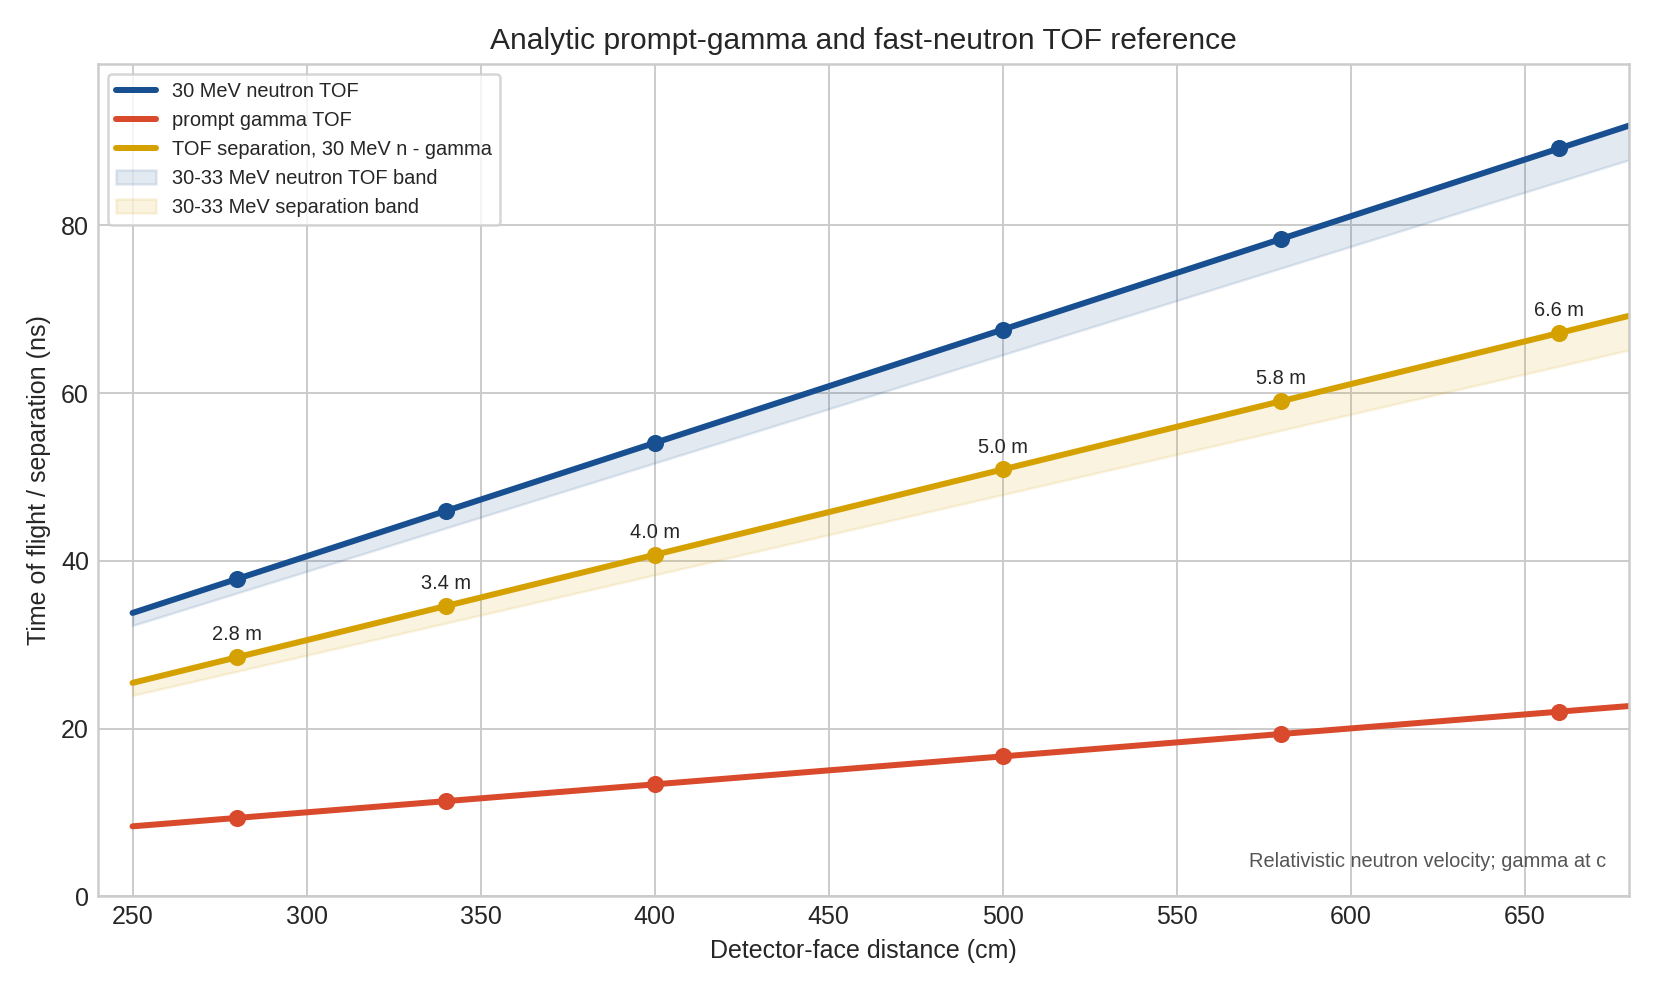
\includegraphics[width=0.92\textwidth]{figures/Gamma_Neutron_deltaTOF_30MeV_reference_positions.png}
\caption{Analytical prompt-gamma and fast-neutron time-of-flight reference for the NCAL position scan. The central neutron curve uses \SI{30}{MeV}; the shaded band indicates the small change between \SI{30}{MeV} and \SI{33}{MeV}. The \SI{30}{MeV} choice is a representative fast-neutron reference within the high-energy part of the \SI{35}{MeV} proton-on-beryllium spectrum, not a monoenergetic source assumption.}
\label{fig:gamma-neutron-tof-reference-positions}
\end{figure}

The qualitative motivation for this treatment is visible directly in the folded RF phase-versus-ToT products. Figure~\ref{fig:position-scan-phase-tot-panel} collects representative channel-2 maps from the completed position-scan runs, with the detector-face distance stated explicitly above each panel. The compact prompt-like island remains narrow in phase and ToT, while the broader neutron-dominated structure changes its relative timing as the detector distance is varied. The figure is included to show the observable space in which the later template or mixture analysis must operate; the different panels should not be read as an absolute yield comparison because the displayed density scales are plot-level renderings.

\begin{landscape}
\begin{figure}[p]
\centering
\begin{minipage}{0.32\linewidth}
\centering
{\small\bfseries Detector face: \SI{2.8}{m}}\\[0.25em]
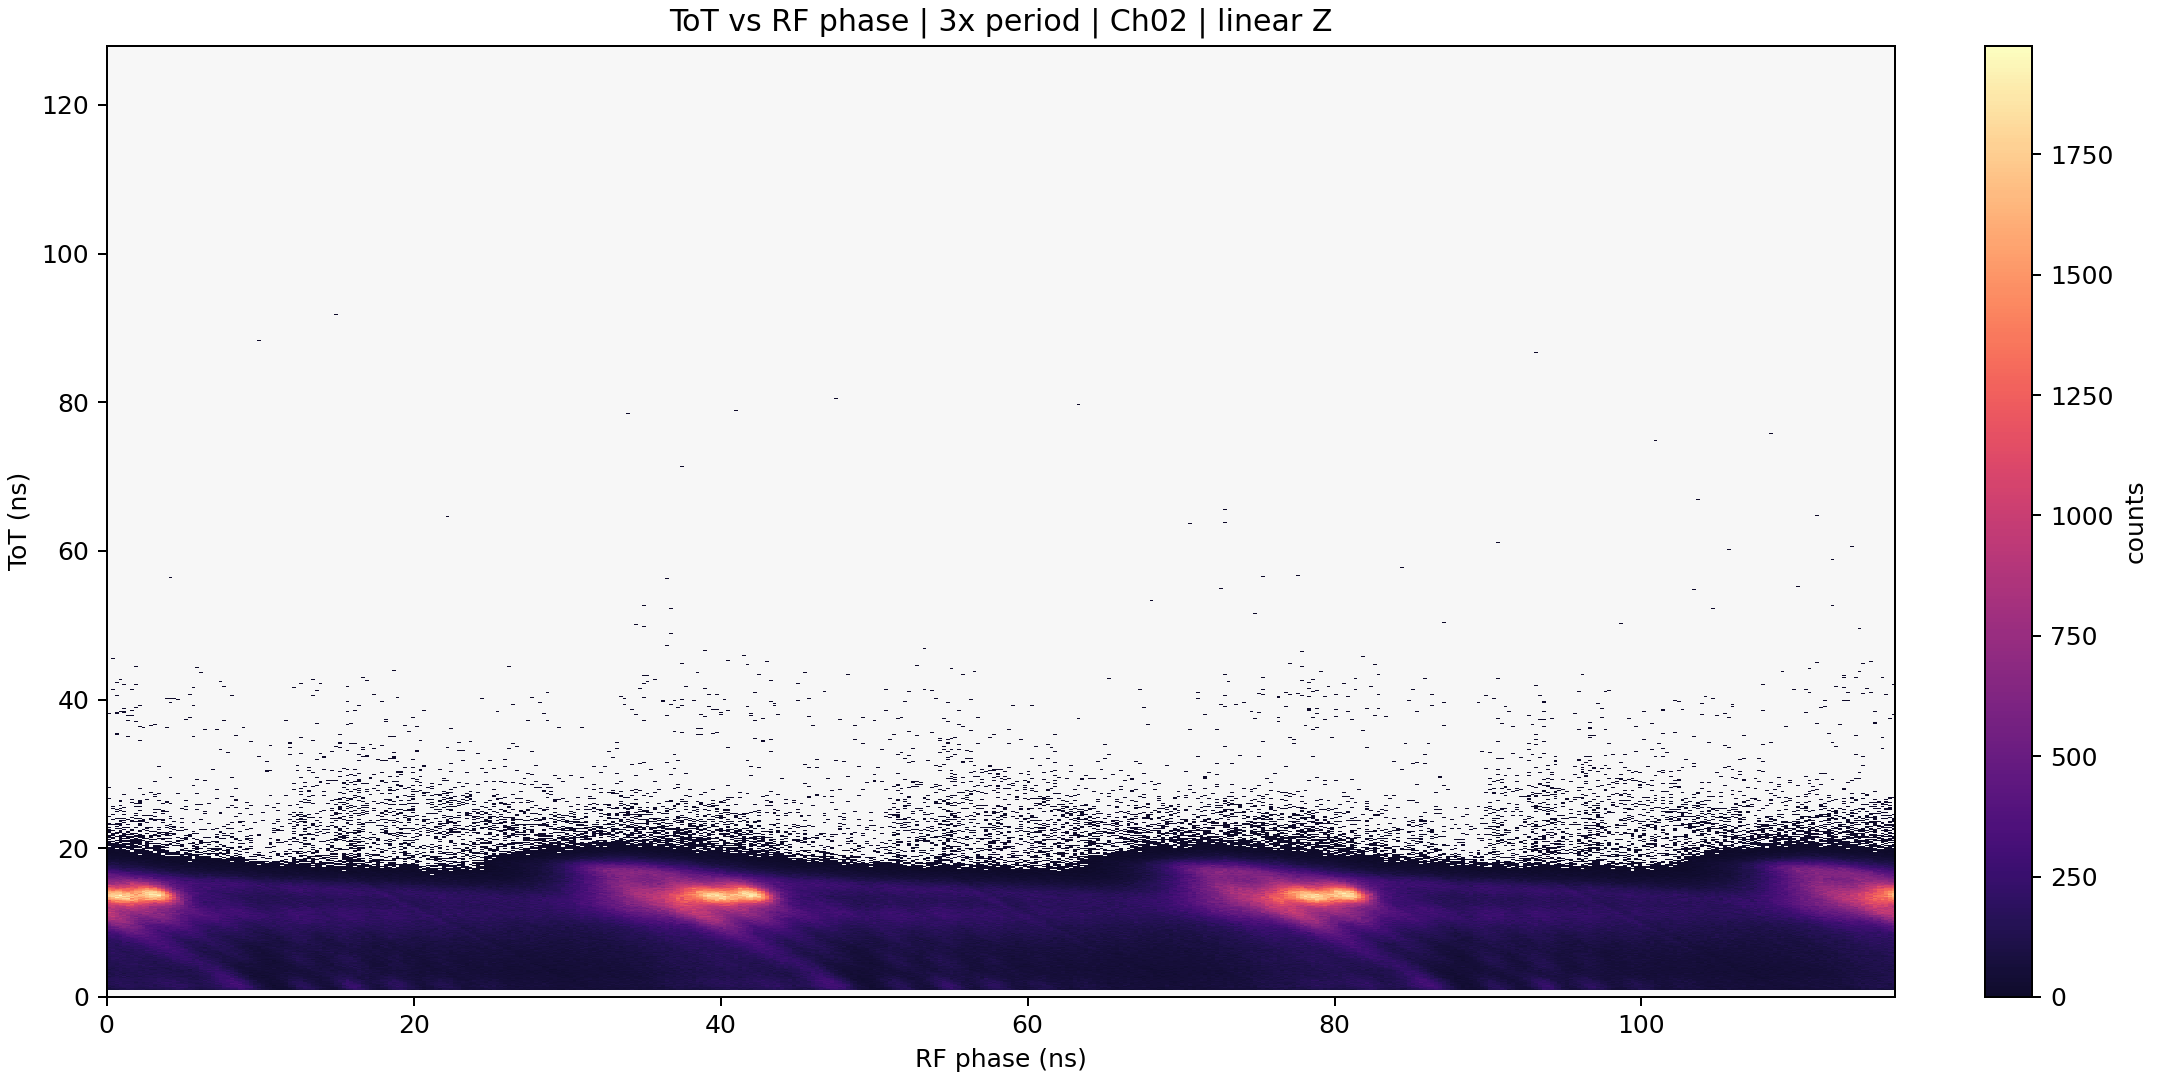
\includegraphics[width=\linewidth]{figures/phase_tot_position_scan/pos_2p8m_ch02_rf_phase_3x_vs_tot.png}
\end{minipage}\hfill
\begin{minipage}{0.32\linewidth}
\centering
{\small\bfseries Detector face: \SI{3.4}{m}}\\[0.25em]
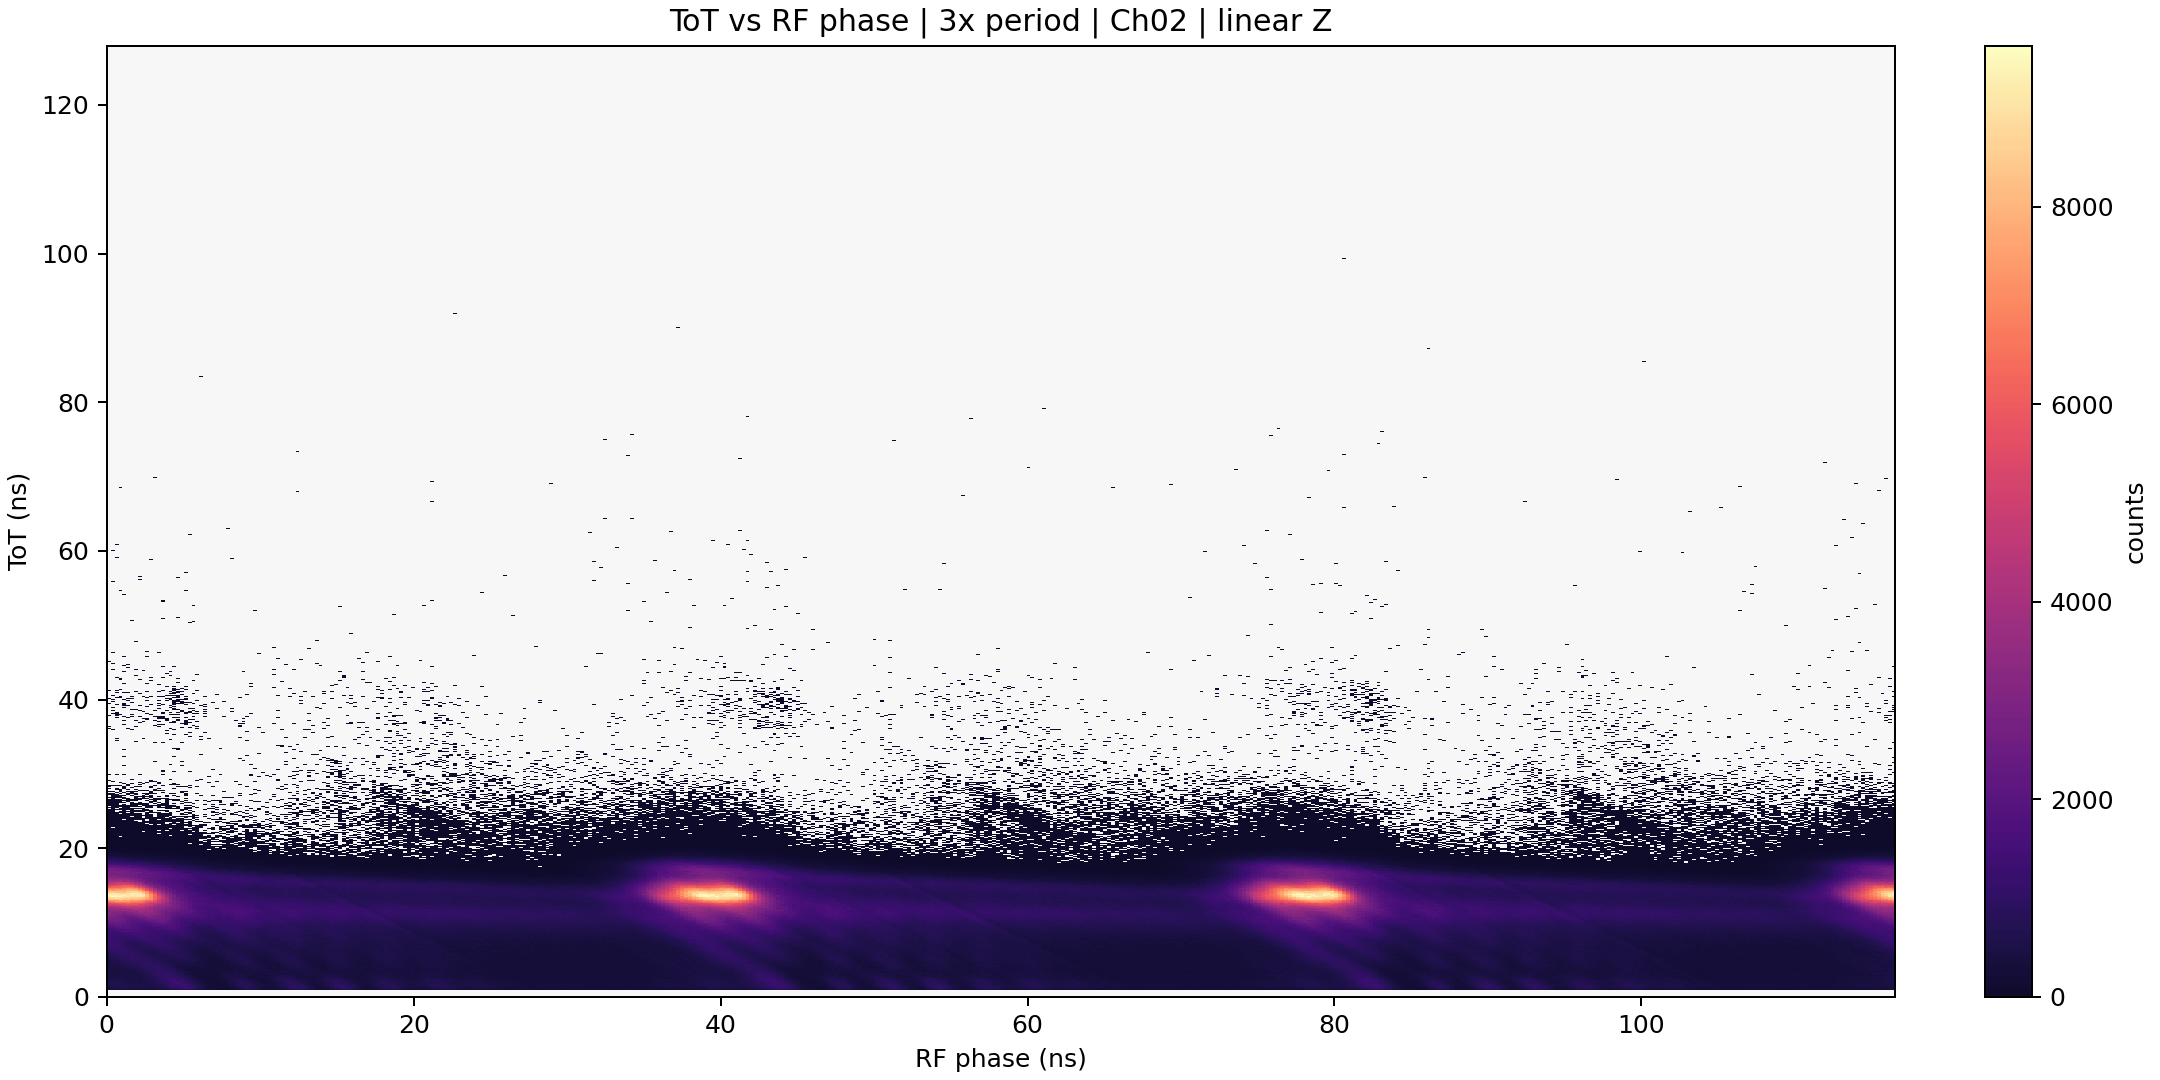
\includegraphics[width=\linewidth]{figures/phase_tot_position_scan/pos_3p4m_ch02_rf_phase_3x_vs_tot.png}
\end{minipage}\hfill
\begin{minipage}{0.32\linewidth}
\centering
{\small\bfseries Detector face: \SI{4.0}{m}}\\[0.25em]
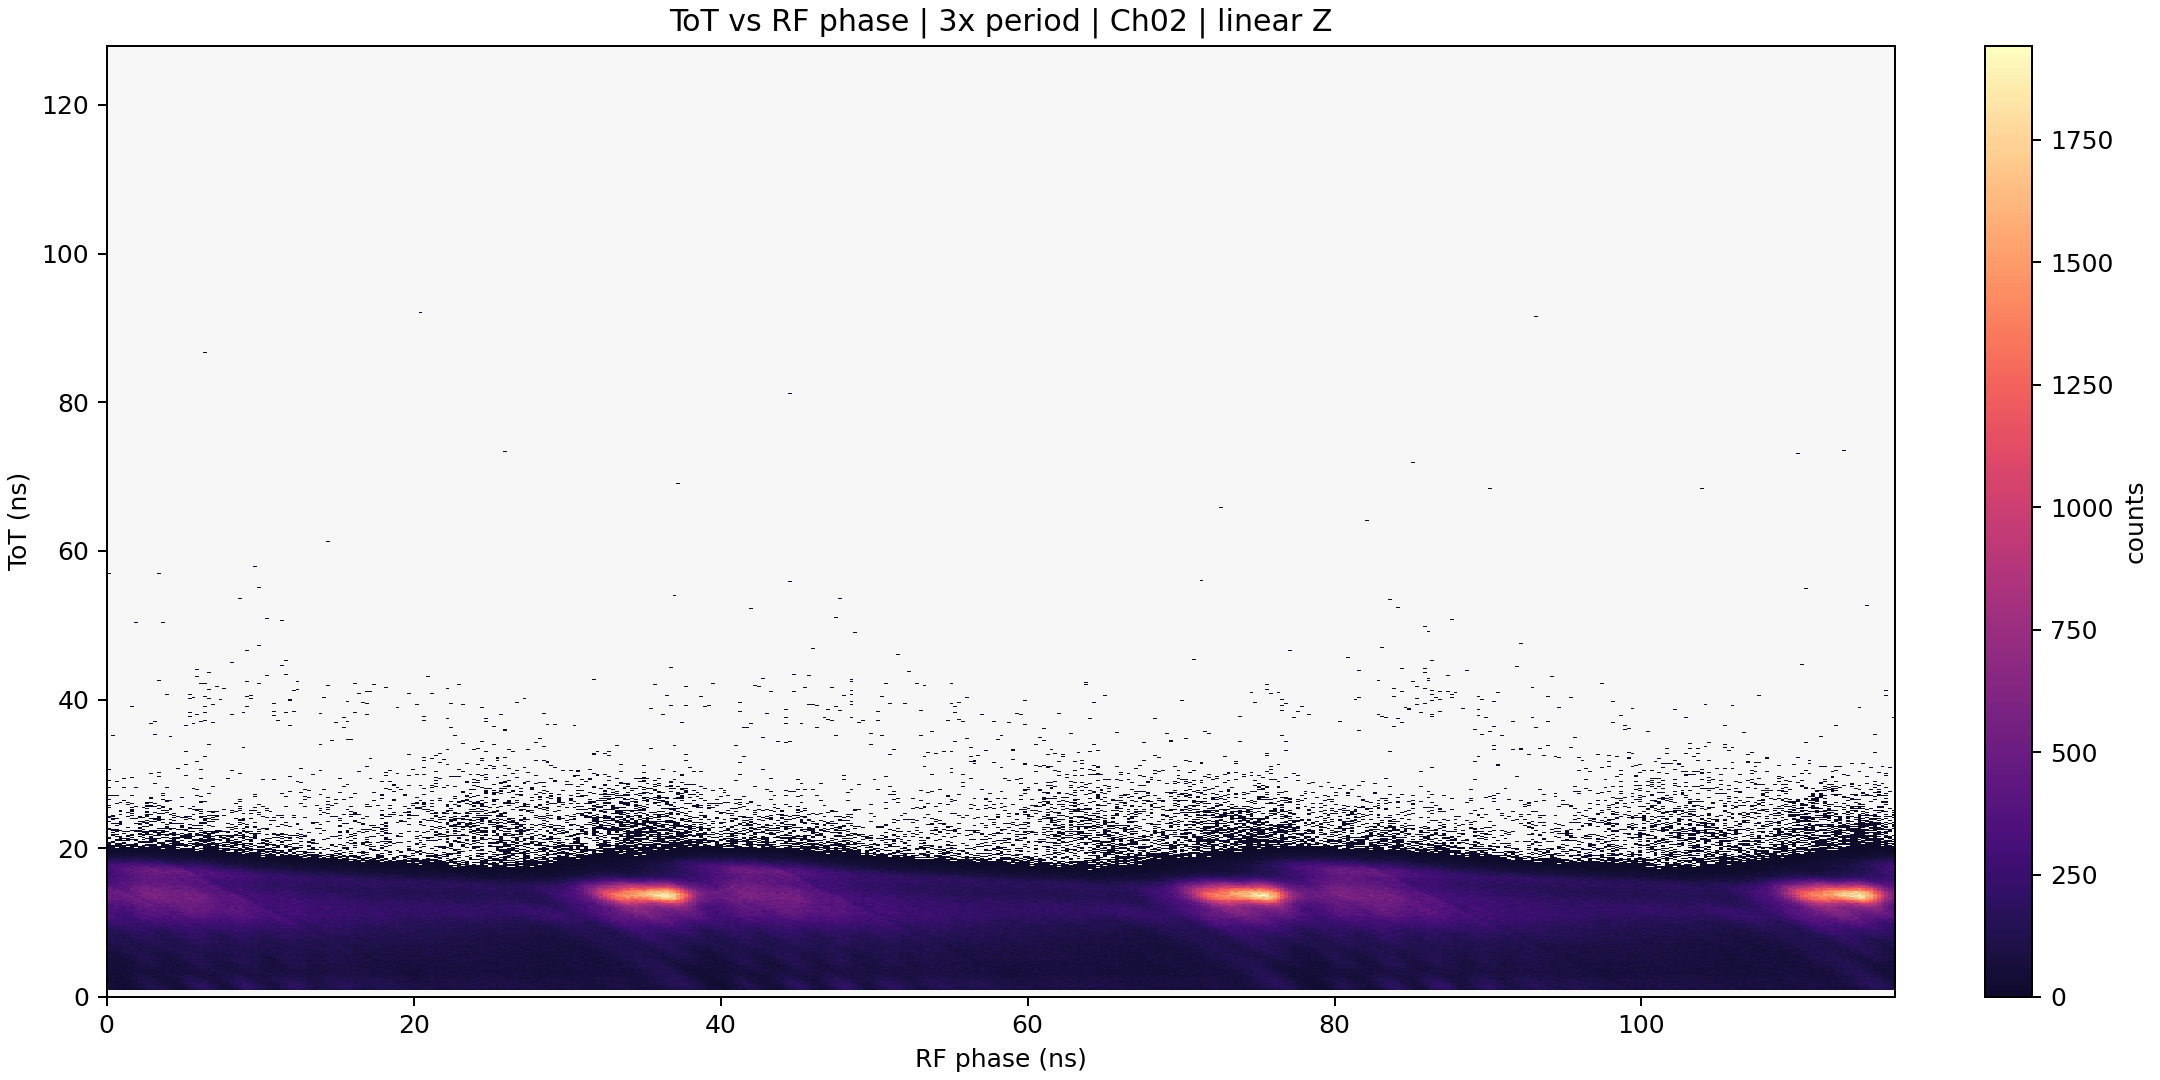
\includegraphics[width=\linewidth]{figures/phase_tot_position_scan/pos_4p0m_ch02_rf_phase_3x_vs_tot.png}
\end{minipage}

\vspace{0.5cm}

\begin{minipage}{0.32\linewidth}
\centering
{\small\bfseries Detector face: \SI{5.0}{m}}\\[0.25em]
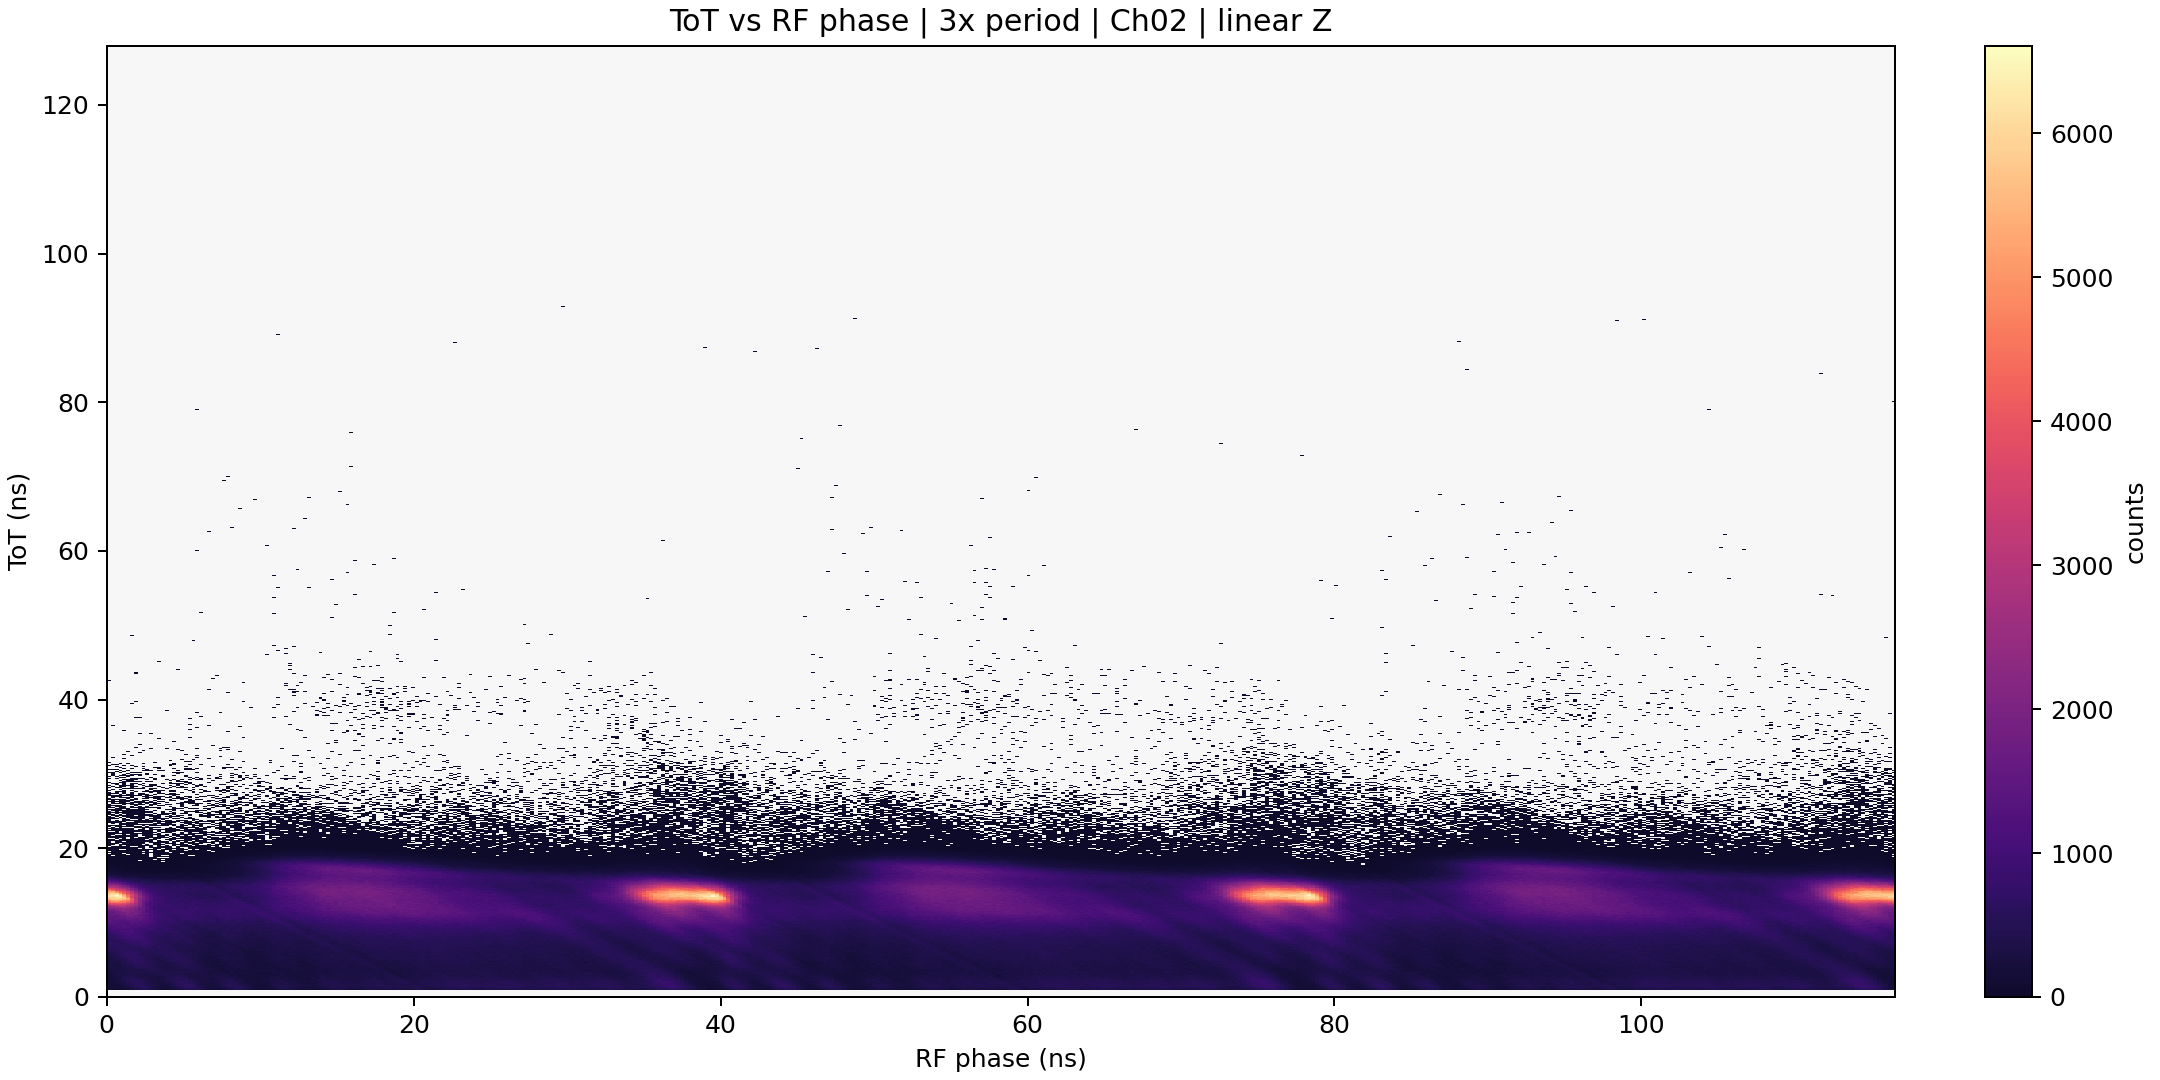
\includegraphics[width=\linewidth]{figures/phase_tot_position_scan/pos_5p0m_ch02_rf_phase_3x_vs_tot.png}
\end{minipage}\hfill
\begin{minipage}{0.32\linewidth}
\centering
{\small\bfseries Detector face: \SI{5.8}{m}}\\[0.25em]
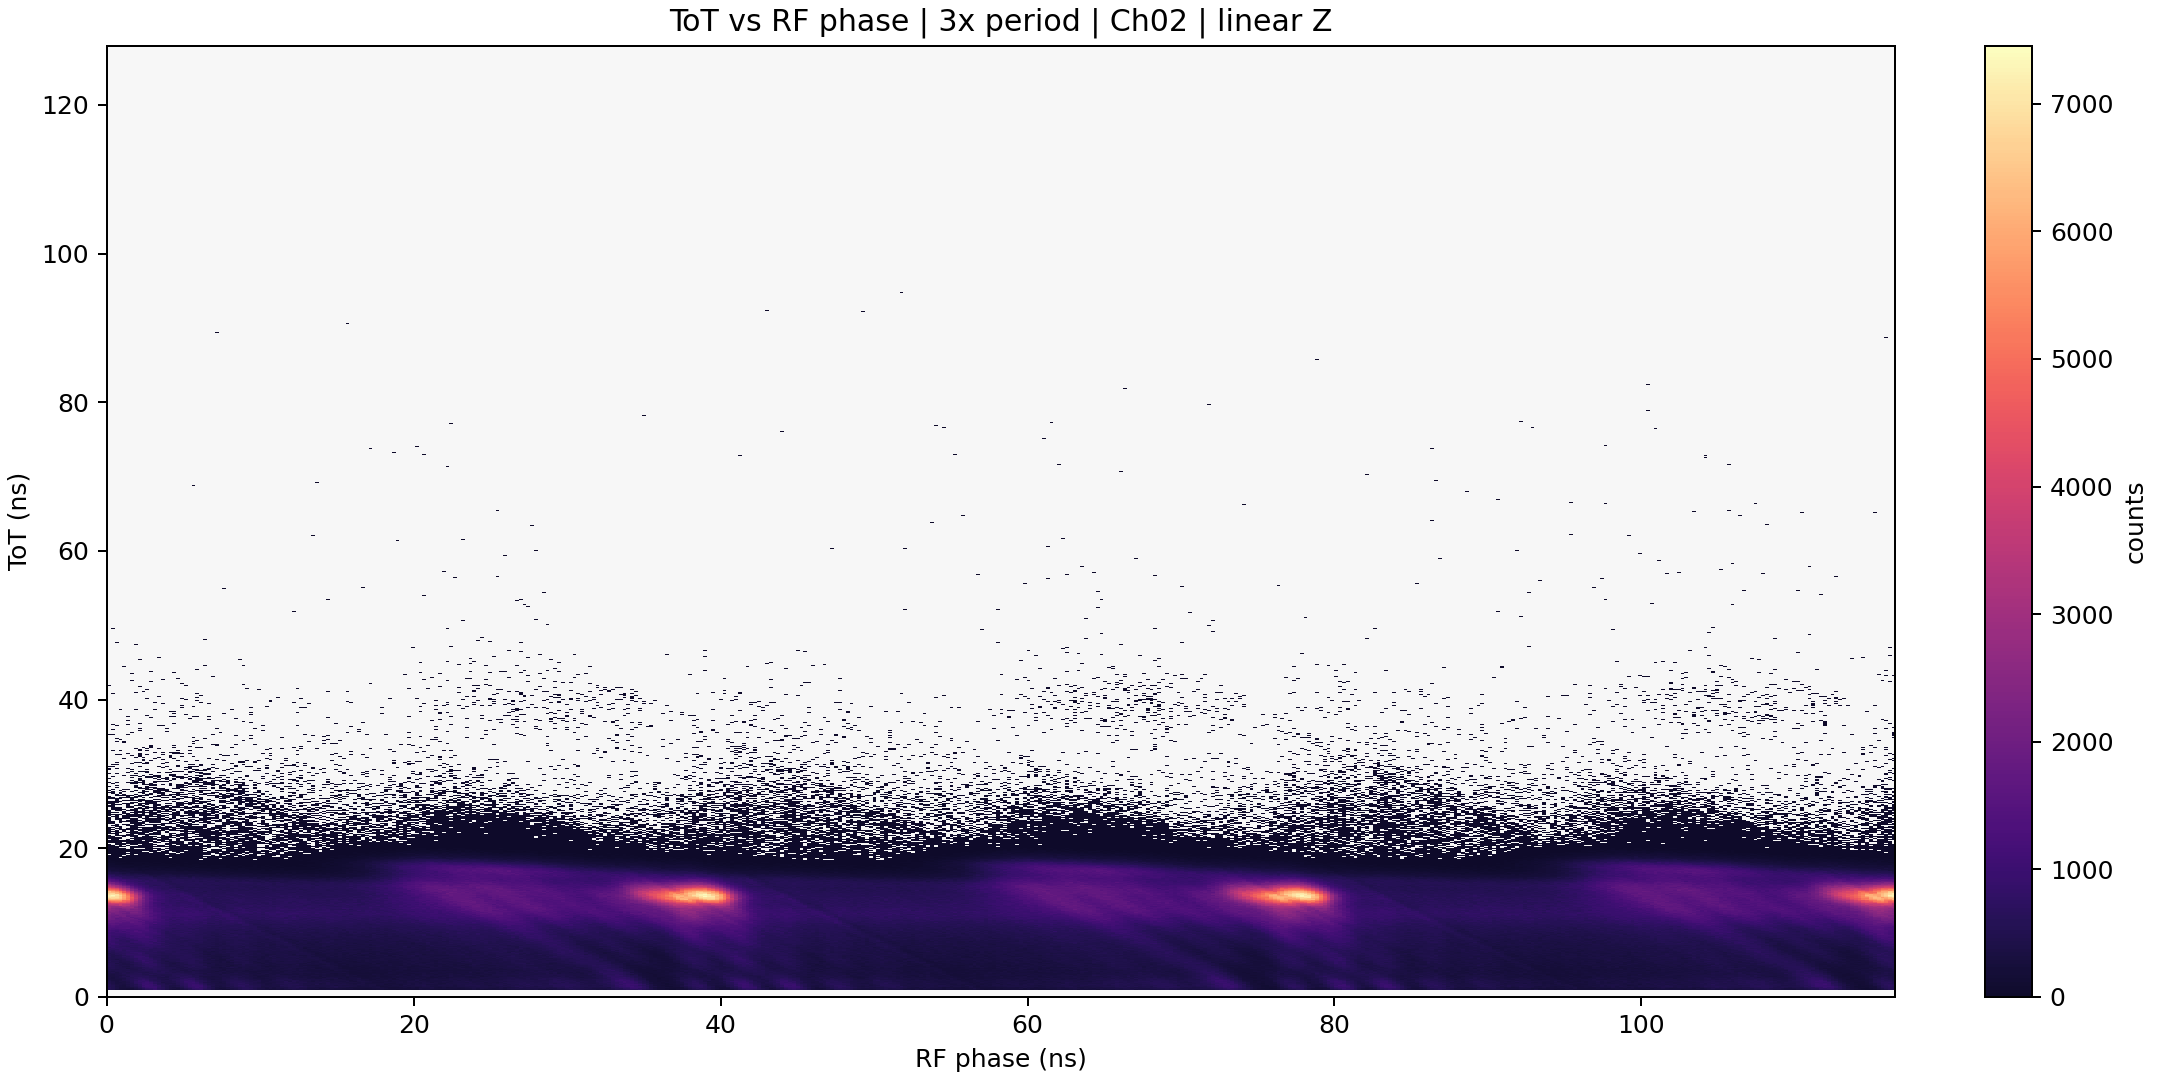
\includegraphics[width=\linewidth]{figures/phase_tot_position_scan/pos_5p8m_ch02_rf_phase_3x_vs_tot.png}
\end{minipage}\hfill
\begin{minipage}{0.32\linewidth}
\centering
{\small\bfseries Detector face: \SI{6.6}{m}}\\[0.25em]
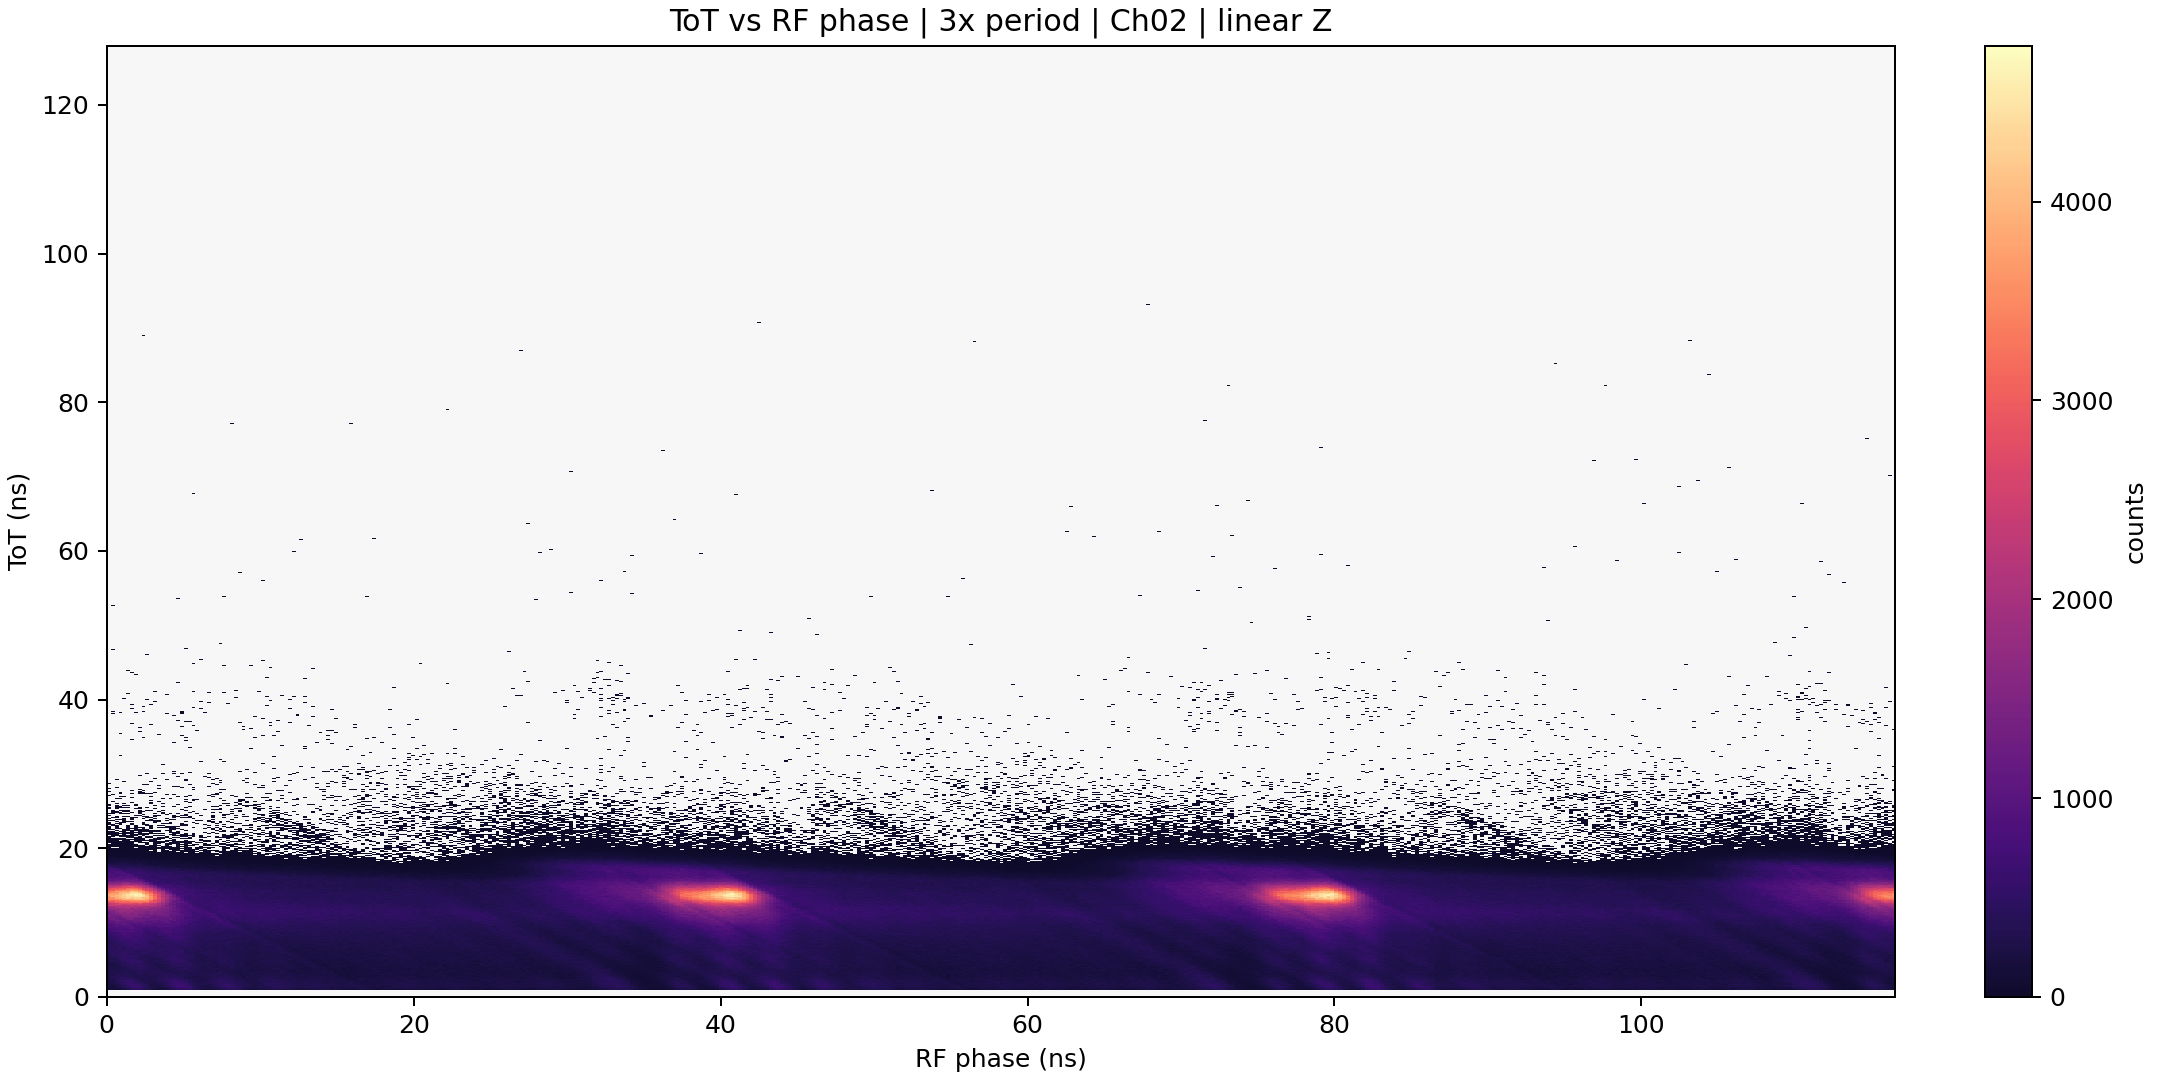
\includegraphics[width=\linewidth]{figures/phase_tot_position_scan/pos_6p6m_ch02_rf_phase_3x_vs_tot.png}
\end{minipage}
\caption{Position-scan view of NCAL channel 2 in folded RF phase and time-over-threshold. Each panel shows the same observable space over three RF periods for a different detector-face distance. The panels motivate the later gamma--neutron separation strategy: at some positions the compact prompt-like island is visibly separated from the broader neutron-dominated distribution, while in overlap regions the event content must be treated as a statistical mixture rather than by unique hit-by-hit labels. The \SI{4.0}{m} panel uses the completed \texttt{NCAL\_20us\_Pos\_4m\_0001} run.}
\label{fig:position-scan-phase-tot-panel}
\end{figure}
\end{landscape}

\chapter{Commissioning and First Validation Workflow}

\section{Purpose of the next work package}

Once stable communication with the DT5725S has been established, the next work package is no longer device discovery but controlled validation. The practical objective is to produce a small set of well-documented reference runs that can be compared later against detector changes, threshold adjustments, firmware changes, or analysis updates. In other words, the transition from ``the board can be opened'' to ``the readout chain is scientifically usable'' requires a reproducible workflow rather than an isolated successful test.

For the present campaign, this next step is especially important because the DAQ chain is expected to support later detector-comparison work and eventual neutron-beam measurements. A reference validation dataset should therefore be treated as an intermediate deliverable in its own right. It anchors later decisions on channel mapping, operating thresholds, pulse polarity, firmware choice, and file-format handling.

\section{Recommended validation sequence}

The initial validation sequence should remain deliberately simple. First, a short pedestal or no-source run should be recorded to document the electronic baseline, pickup environment, and spontaneous trigger behavior. Second, a single detector channel should be connected and validated under the same DAQ settings used during board discovery, so that waveform stability and trigger-rate response can be checked without the ambiguity introduced by multi-channel operation. Third, only after this single-channel behavior is stable should threshold adjustments or additional detector channels be introduced.

For the current DT5725S configuration with DPP-PSD firmware and \textit{CoMPASS}, the minimum acceptance test for a reference run is straightforward: the board must be rediscovered after a fresh start, a selected channel must produce a stable rate and visible pulses, and the saved data file must be consistent with the configuration used during acquisition. If any of these conditions fails, the run should be classified as a commissioning test rather than as a physics-quality reference run.

Where detector conditions permit it, a very small threshold scan is already useful at this stage. Even a coarse set of operating points can reveal whether the observed rate is dominated by electronic noise, low-amplitude background, or clearly resolved detector pulses. This is more informative than relying on a single visually satisfactory setting, and it provides a first quantitative handle on the stability margin of the chosen operating point.

\section{Run record and promotion criteria}

Each accepted validation run should preserve more than the raw event file alone. At minimum, the run record should include the saved \textit{CoMPASS} configuration, the board serial number, the firmware identifiers reported by the CAEN libraries, the driver version or package used on the acquisition PC, the active channel list, the detector connected to each channel, the applied threshold and polarity settings, and a short operator note stating the source or pulser condition. This information is lightweight to archive, but it is essential if later discrepancies between runs are to be interpreted correctly.

Promotion from validation mode to routine data taking should require three conditions. First, board communication must remain stable across repeated restarts of both the software and the device. Second, the observed count rate and displayed pulses must remain consistent over a run long enough to exclude a transient startup effect. Third, the complete acquisition state must be reproducible by another operator using only the stored configuration and laboratory notes. If these conditions are met, subsequent measurements can be interpreted as detector studies rather than as continued infrastructure debugging.

This work package also defines the point at which a future branch in the DAQ strategy becomes meaningful. If the reference runs show that the DPP-PSD configuration already provides the observables needed for detector discrimination and timing studies, then the present firmware can be retained for the next stage. If, however, the later analysis requires full trace-level treatment of baselines, charge integration windows, or pulse-shape development, then the justified next step is a planned transition to the x725S waveform-recording firmware together with a waveform-oriented acquisition program.

\bibliographystyle{plainnat}
\bibliography{references}

\end{document}